% !TeX root = ../main.tex
\chapter{Tolerancia a las degradaciones del canal}
\label{cap:tolerancias}

\section{Introducci\'on}
\label{sec:tol-intro}

En este cap\'itulo se eval\'uan los l\'imites de operaci\'on del receptor
frente a cada una de las degradaciones consideradas. Para cada deterioro se
barre la variable que lo controla, aumentando su magnitud hasta que el
receptor deja de cumplir el requisito de BER, y se identifica el mecanismo
que produce la falla.

Se tiene dos objetivos. Por un lado, entender qu\'e limita el desempe\~no en
cada caso. Por otro, cuantificar el margen que queda entre el l\'imite medido
y el valor que el enlace realmente impone, calculado en el \cref{cap:canal}.
Los resultados se re\'unen en una tabla al final del cap\'itulo.

\section{Metodolog\'ia}
\label{sec:tol-metodologia}

\paragraph{M\'etrica de evaluaci\'on:}
Para evaluar la tolerancia del receptor se utiliza la magnitud del vector de
error, EVM, tomada siempre sobre la polarizaci\'on de peor desempe\~no y no
sobre el promedio de las dos. Se toma la peor porque algunas fallas del
receptor afectan a una sola polarizaci\'on, y promediarlas disimular\'ia el colapso.

\paragraph{Estimaci\'on de la penalidad de OSNR:}
La penalidad asociada a un deterioro es el incremento de OSNR necesario para
mantener el desempe\~no en el umbral HD-FEC. Determinarla de forma directa
obligar\'ia a correr un barrido de OSNR completo en cada punto, con un costo
de simulaci\'on muy alto. En su lugar se la estima a partir del EVM,
aprovechando que en QPSK con ruido gaussiano aditivo vale
$\EVM^{2} = 1/\mathrm{SNR}$, con el EVM normalizado al valor eficaz de la
constelaci\'on de referencia.

La conversi\'on tiene dos pasos. Primero se separa en cuadratura lo que
aporta el deterioro de lo que aporta el ruido \'optico, que ya estaba en el
punto limpio. Despu\'es se convierte esa fracci\'on del presupuesto de error
en decibeles.
\begin{equation}
  \EVM_{\mathrm{imp}}^{2} = \EVM_{\mathrm{med}}^{2} - \EVM_{\mathrm{limpio}}^{2},
  \qquad
  \mathcal{P}\,[\si{\dB}] = -10\log_{10}\!
  \left[1 - \left(\frac{\EVM_{\mathrm{imp}}}{\EVM_{\mathrm{th}}}\right)^{2}\right],
  \label{eq:tol-penalidad}
\end{equation}
con $\EVM_{\mathrm{th}} = \SI{37.46}{\percent}$ el EVM que corresponde al
umbral HD-FEC.

\section{Offset de frecuencia Doppler}
\label{sec:tol-doppler}

El desplazamiento Doppler introduce una diferencia de frecuencia entre la
portadora \'optica recibida y el oscilador local del receptor, que el DSP
tiene que estimar y compensar. En la \cref{eq:requisito-captura} se
estableci\'o un requisito de captura de \SI{\pm 6.0}{\giga\hertz} para el
enlace LEO--GEO. En esta secci\'on se eval\'ua en simulaci\'on el rango de
frecuencias que el receptor puede compensar, y se verifica su cumplimiento
para las tres tasas de s\'imbolo consideradas.

\begin{figure}[H]
  \centering
  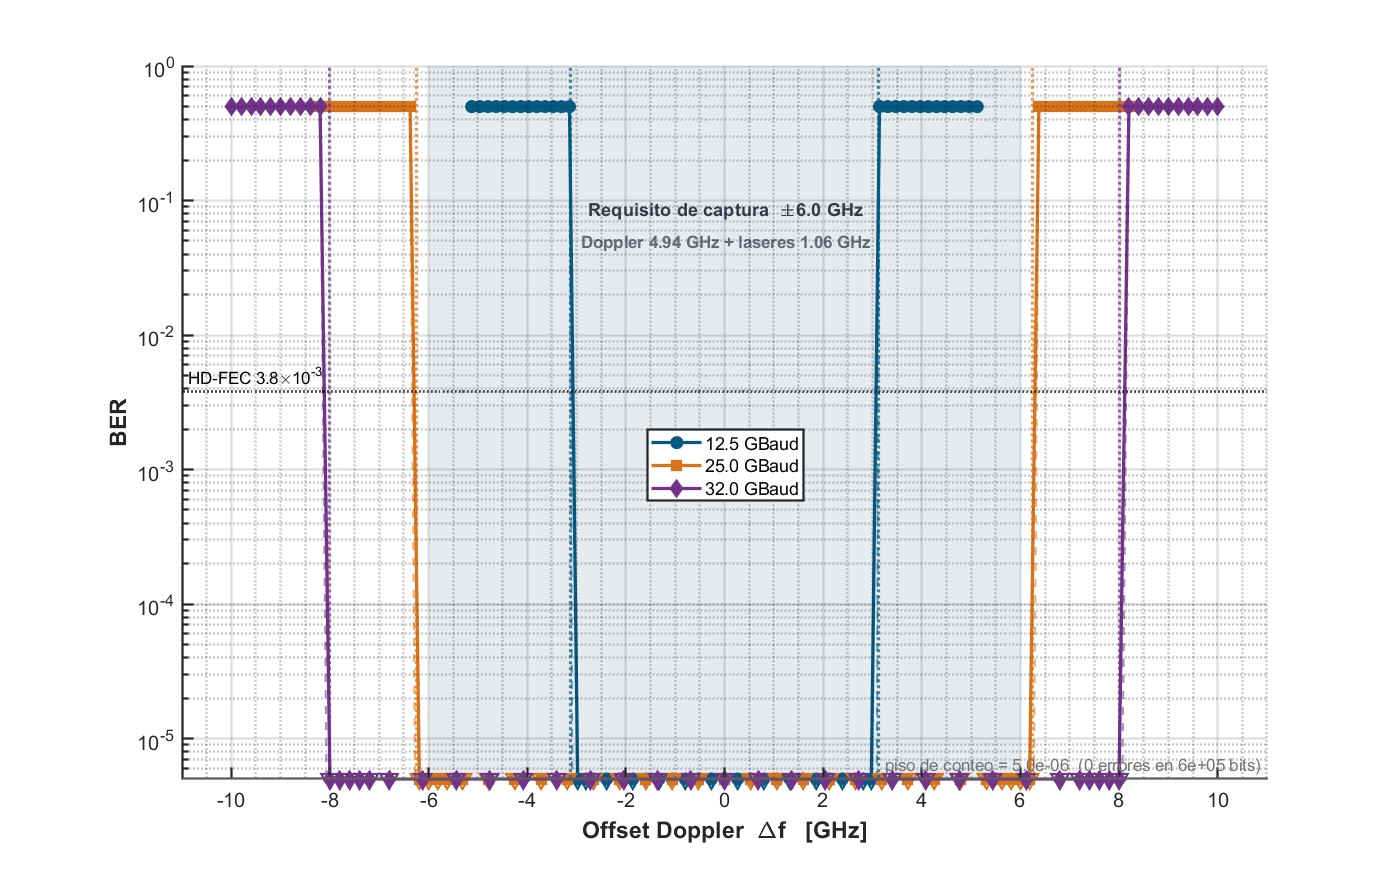
\includegraphics[width=0.92\textwidth]{figuras/EfectoDopplerFiguraFinalSimulacion.jpg}
  \caption[Tolerancia al offset Doppler en simulaci\'on]{%
    BER contra offset Doppler para las tres tasas de s\'imbolo para una OSNR
    fija, en simulaci\'on. La franja sombreada es el requisito de captura del
    enlace, \SI{\pm 6.0}{\giga\hertz}. La l\'inea de trazos es el umbral
    HD-FEC.}
  \label{fig:tol-doppler-sim}
\end{figure}

La \cref{fig:tol-doppler-sim} muestra que la BER se mantiene
aproximadamente constante dentro de un intervalo de frecuencias, a partir del
cual sube de forma abrupta hasta valores cercanos a \num{0.5}, sin
degradaci\'on gradual.

Los l\'imites de captura obtenidos son de \SI{\pm 3.1}{\giga\hertz} a
\SI{12.5}{\giga\baud}, \SI{\pm 6.25}{\giga\hertz} a \SI{25}{\giga\baud} y
\SI{\pm 8.0}{\giga\hertz} a \SI{32}{\giga\baud}, es decir $\Rs/4$ en las
tres. El mecanismo est\'a explicado en la \cref{sec:dsp-frec-limite}. El
estimador trabaja sobre la se\~nal elevada a la cuarta potencia, de modo que
el offset aparece como un tono en $4\Df$. La se\~nal est\'a muestreada a dos
muestras por s\'imbolo, as\'i que $F_s = 2\Rs$ y la frecuencia de Nyquist es
$F_s/2 = \Rs$. La igualdad $4\Df = \Rs$ se alcanza en $\Df = \Rs/4$, y por
encima de ese valor el tono se pliega y el estimador deja de identificar
correctamente el offset.

El mecanismo se puede observar de forma directa mirando qu\'e frecuencia
entrega el estimador. La \cref{fig:tol-frecuencia-estimada} compara la
estimaci\'on contra el offset realmente aplicado, para las mismas tres tasas
de s\'imbolo.

\begin{figure}[H]
  \centering
  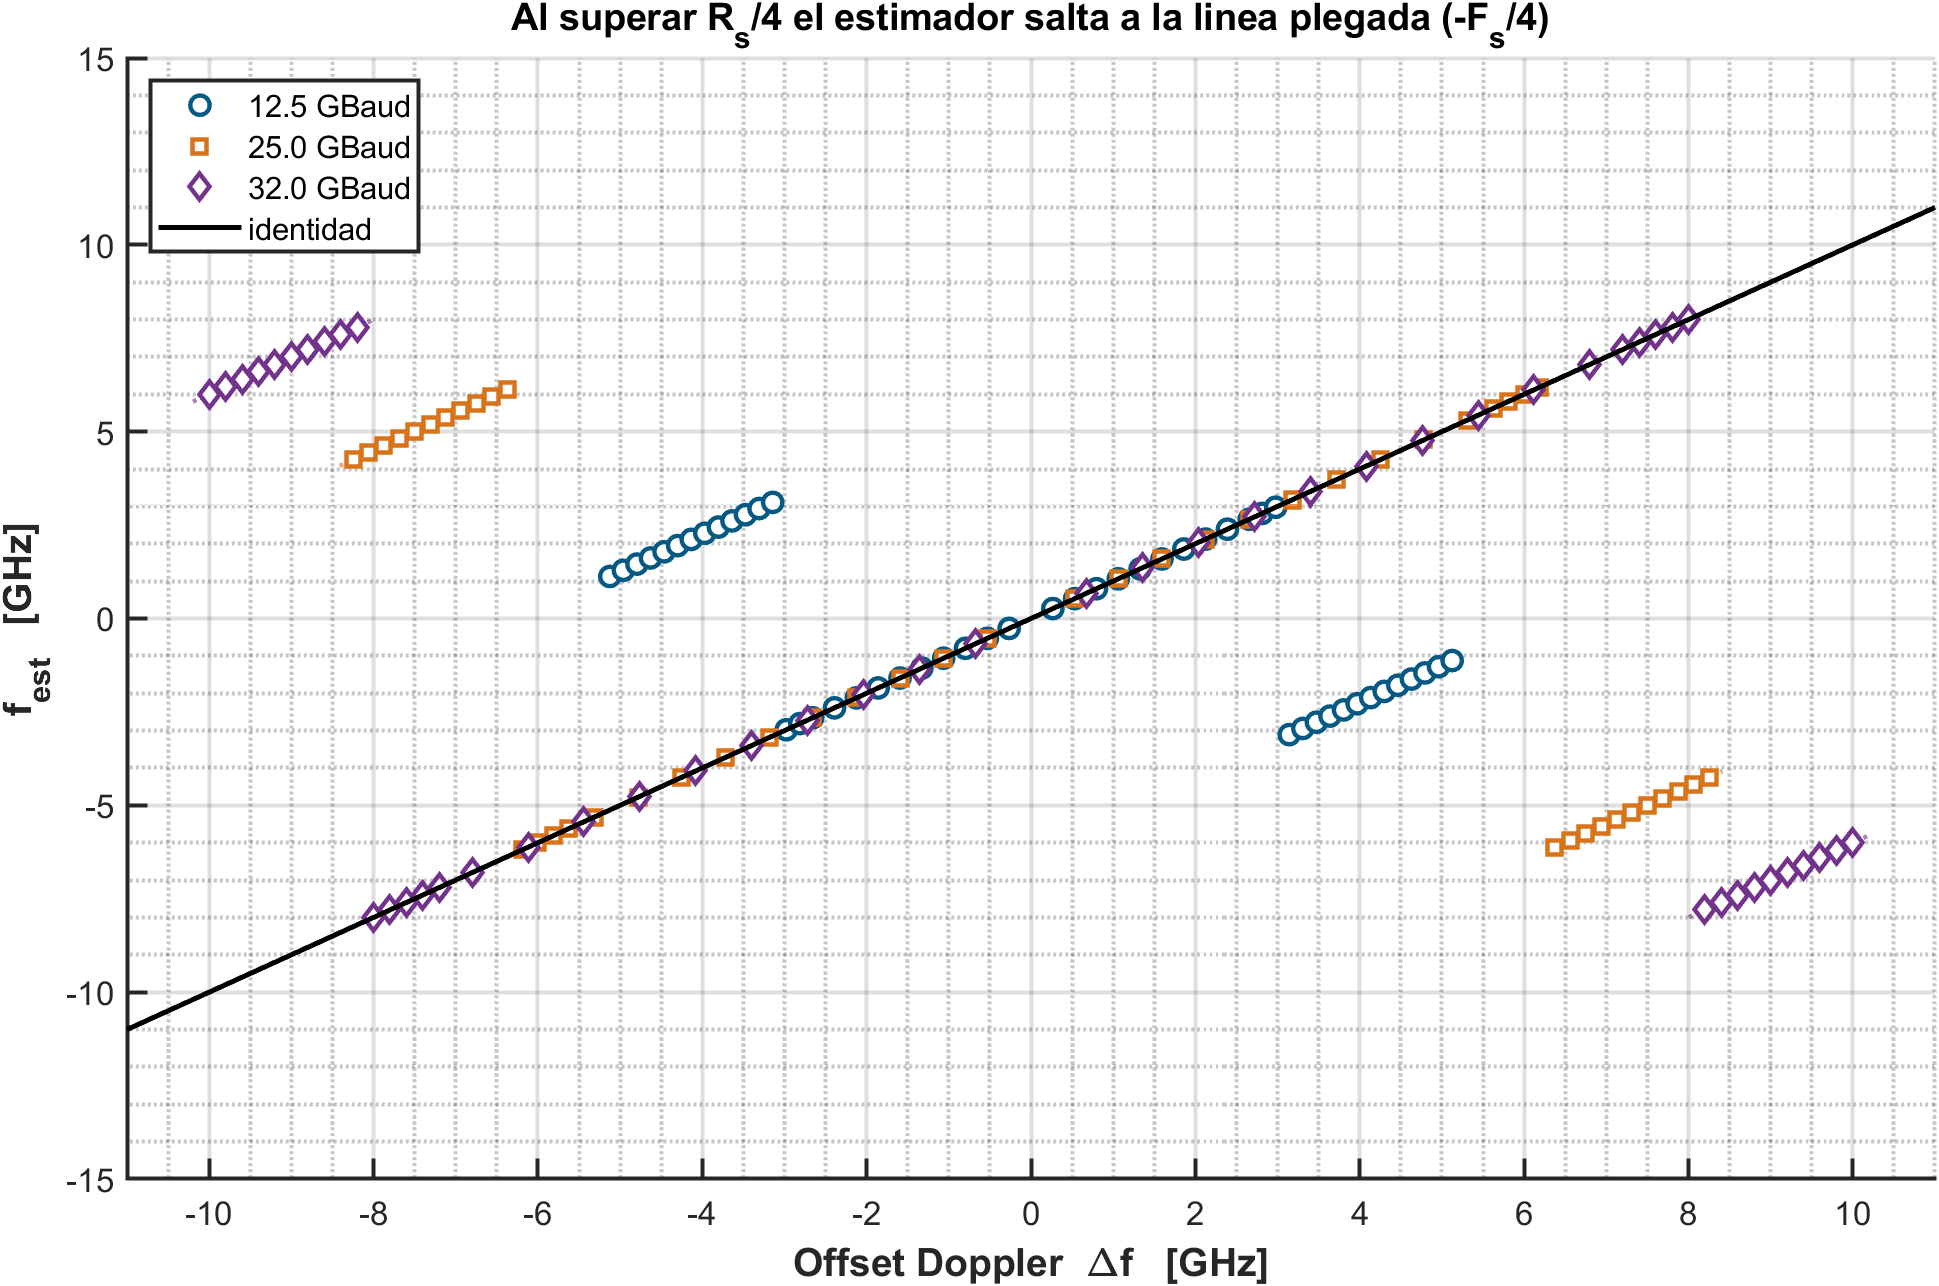
\includegraphics[width=0.92\textwidth]{figuras/tol_frecuencia_estimada.png}
  \caption[Frecuencia estimada contra offset aplicado]{%
    Frecuencia estimada por el bloque de recuperaci\'on en funci\'on del offset
    aplicado, para las tres tasas de s\'imbolo. La recta negra es la
    identidad. Mientras el tono cae dentro de la banda de Nyquist la
    estimaci\'on la sigue. Pasado $\Rs/4$ el tono se pliega y la estimaci\'on
    salta a una segunda recta, paralela a la primera y desplazada en
    $\Rs/2$.}
  \label{fig:tol-frecuencia-estimada}
\end{figure}

Mientras el tono cae dentro de la banda, la estimaci\'on sigue la identidad
en las tres tasas. Pasado $\Rs/4$ no se vuelve err\'atica sino que salta a un
valor determinado,
\begin{equation}
  f_{\mathrm{est}} = \Df - \frac{\Rs}{2},
  \label{eq:tol-plegado}
\end{equation}
que es la posici\'on del tono plegado. El salto escala con la tasa de
s\'imbolo, de \SI{6.25}{\giga\hertz} a \SI{12.5}{\giga\baud} a
\SI{16}{\giga\hertz} a \SI{32}{\giga\baud}, lo que confirma que el l\'imite
de captura lo fija d\'onde cae el tono dentro de la banda de Nyquist.

\begin{table}[htbp]
  \centering

  \begin{tabular}{lccc}
    \toprule
     $\Rs$ & $\Rs/4$ & Simulaci\'on & Margen \\
    \midrule
    \SI{12.5}{\giga\baud} & \SI{3.125}{\giga\hertz} & \SI{\pm 3.1}{\giga\hertz}  & \SI{-2.9}{\giga\hertz}  \\
    \SI{25}{\giga\baud}   & \SI{6.25}{\giga\hertz}  & \SI{\pm 6.25}{\giga\hertz} & \SI{+0.25}{\giga\hertz} \\
    \SI{32}{\giga\baud}   & \SI{8.0}{\giga\hertz}   & \SI{\pm 8.0}{\giga\hertz}  & \SI{+2.0}{\giga\hertz}  \\
    \bottomrule
  \end{tabular}
  \caption[Ventana de captura de Doppler]{%
    Ventana de captura medida en simulaci\'on contra el l\'imite te\'orico
    $\Rs/4$. La \'ultima columna es la diferencia con el requisito de captura
    del enlace, \SI{\pm 6.0}{\giga\hertz}.}
  \label{tab:tol-doppler}
\end{table}

La tolerancia al offset crece con la tasa de s\'imbolo. A
\SI{12.5}{\giga\baud} el rango de captura no alcanza para cubrir el requisito
de \SI{\pm 6.0}{\giga\hertz}. A \SI{25}{\giga\baud} el requisito se cumple,
aunque con un margen reducido de \SI{0.25}{\giga\hertz}. A
\SI{32}{\giga\baud} el margen es de \SI{2.0}{\giga\hertz}, de modo que el
receptor cumple con holgura.

\subsection{Dependencia con la relaci\'on se\~nal-ruido}
\label{sec:tol-doppler-osnr}

Para evaluar la influencia del ruido \'optico sobre el rango de captura, se
repiti\'o el barrido de offset a \SI{32}{\giga\baud} para doce valores de
OSNR entre \SI{10}{\dB} y \SI{21}{\dB}.

\begin{figure}[H]
  \centering
  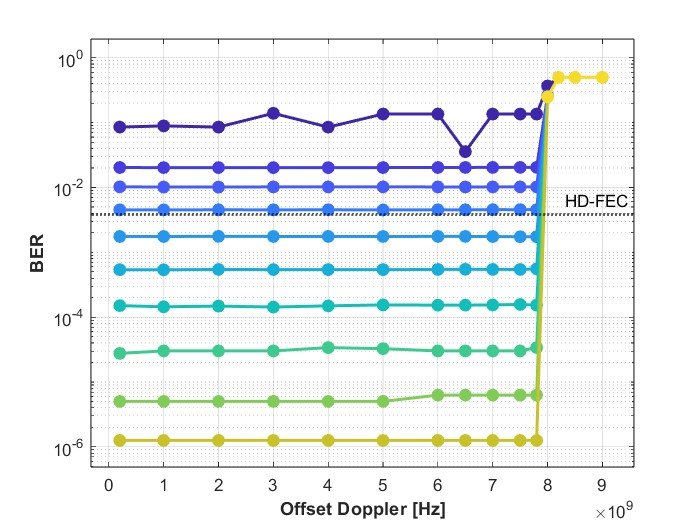
\includegraphics[width=0.92\textwidth]{figuras/tol_doppler_osnr.jpg}
  \caption[Offset Doppler contra la familia de OSNR]{%
    BER contra offset Doppler para doce valores de OSNR. El color denota una
    OSNR en pasos de \SI{1}{\dB}, de azul oscuro en \SI{10}{\dB} a amarillo
    en \SI{21}{\dB}. Las curvas se desplazan verticalmente con la OSNR pero
    quiebran todas en el mismo punto.}
  \label{fig:tol-doppler-osnr}
\end{figure}

Como se observa en la \cref{fig:tol-doppler-osnr}, para OSNR entre
\SI{13}{\dB} y \SI{21}{\dB} el receptor funciona hasta
\SI{7.8}{\giga\hertz} y colapsa en \SI{8.0}{\giga\hertz}. El quiebre no se
desplaza con la OSNR y queda en $\Rs/4$ en todos los casos, que es el mismo
plegado de la \cref{fig:tol-frecuencia-estimada}. Al tratarse de un efecto de
muestreo, el nivel de ruido no lo corre. Por debajo de \SI{13}{\dB} se
observan degradaciones adicionales, posiblemente asociadas a dificultades del
lazo de recuperaci\'on de fase.

\section{Tasa de chirp Doppler}
\label{sec:tol-chirp}

El desplazamiento Doppler no es constante a lo largo del pase, porque la
velocidad radial relativa entre los sat\'elites var\'ia. Eso produce una
deriva temporal de la frecuencia recibida, cuya tasa m\'axima se estim\'o en
\SI{6.55}{\mega\hertz\per\second} para las condiciones de vuelo
consideradas. En esta secci\'on se mide cu\'anta deriva tolera el receptor.

\begin{figure}[H]
  \centering
  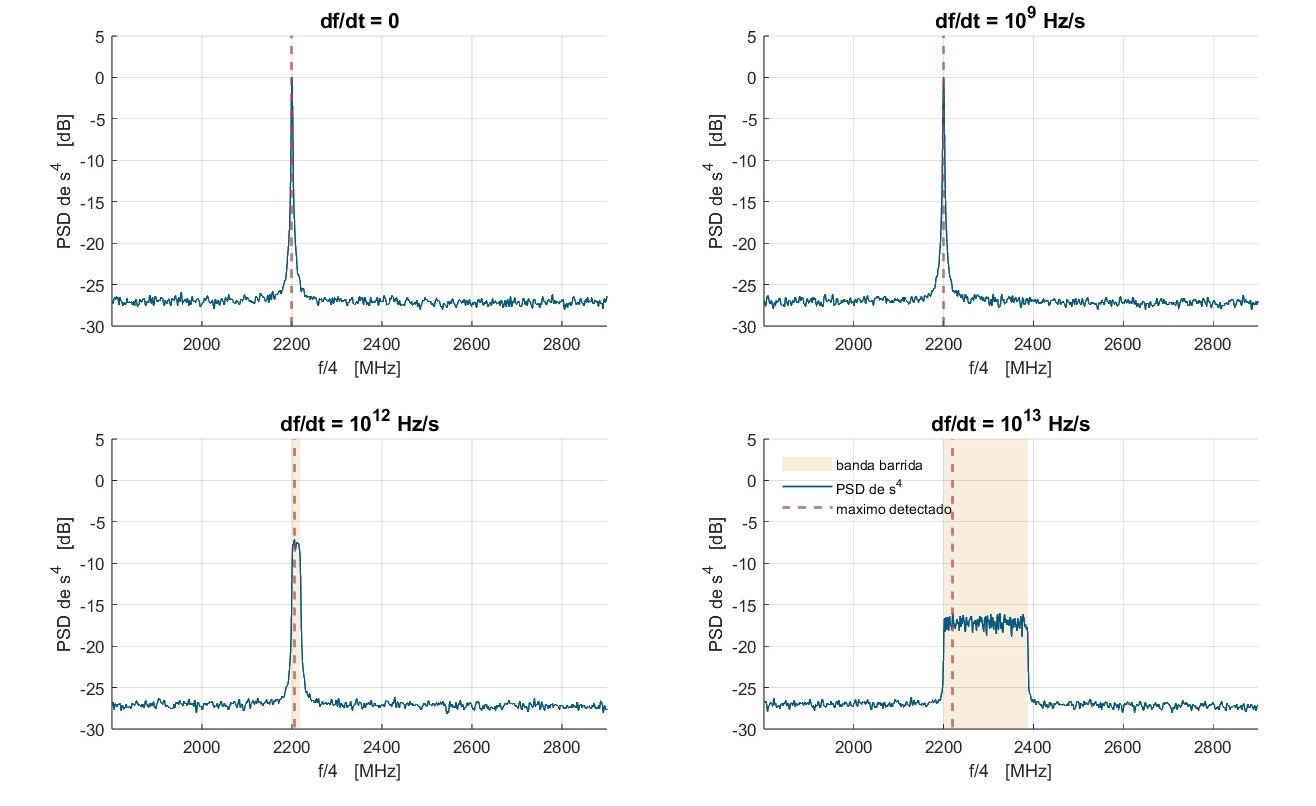
\includegraphics[width=0.92\textwidth]{figuras/EfectoChirp.jpg}
  \caption[Efecto del chirp sobre el espectro de la cuarta potencia]{%
    Densidad espectral de la se\~nal elevada a la cuarta para cuatro tasas de
    chirp, con una ventana de \SI{18.75}{\micro\second} y un offset de
    \SI{2200}{\mega\hertz}. La franja marca la banda barrida durante la
    ventana y la l\'inea de trazos, el m\'aximo que detecta el estimador.}
  \label{fig:tol-efecto-chirp}
\end{figure}

La \cref{fig:tol-efecto-chirp} muestra el efecto del chirp sobre el estimador
de frecuencia. A diferencia de un offset constante, una frecuencia que var\'ia
linealmente con el tiempo ensancha la componente espectral que el estimador
utiliza, porque durante una ventana de duraci\'on $T$ el offset recorre
$\dot f\,T$. Para una tasa de \SI{1e13}{\hertz\per\second} y una ventana de
\SI{18.75}{\micro\second} son \SI{187.5}{\mega\hertz}, y el tono deja de ser
una l\'inea para convertirse en una meseta de \num{2200} a
\SI{2390}{\mega\hertz}. La altura del pico cae en proporci\'on inversa al
ensanchamiento, de \SI{0}{\dB} a \SI{-17}{\dB}, y el estimador se queda con
uno de los m\'aximos dentro de ese rango.

El estimador entrega un \'unico valor de frecuencia para toda la secuencia
procesada, de modo que no puede seguir su variaci\'on temporal. Despu\'es de
la compensaci\'on queda un offset residual que var\'ia a lo largo del
registro, como muestra la \cref{fig:tol-rampa-frecuencia}.

\begin{figure}[H]
  \centering
  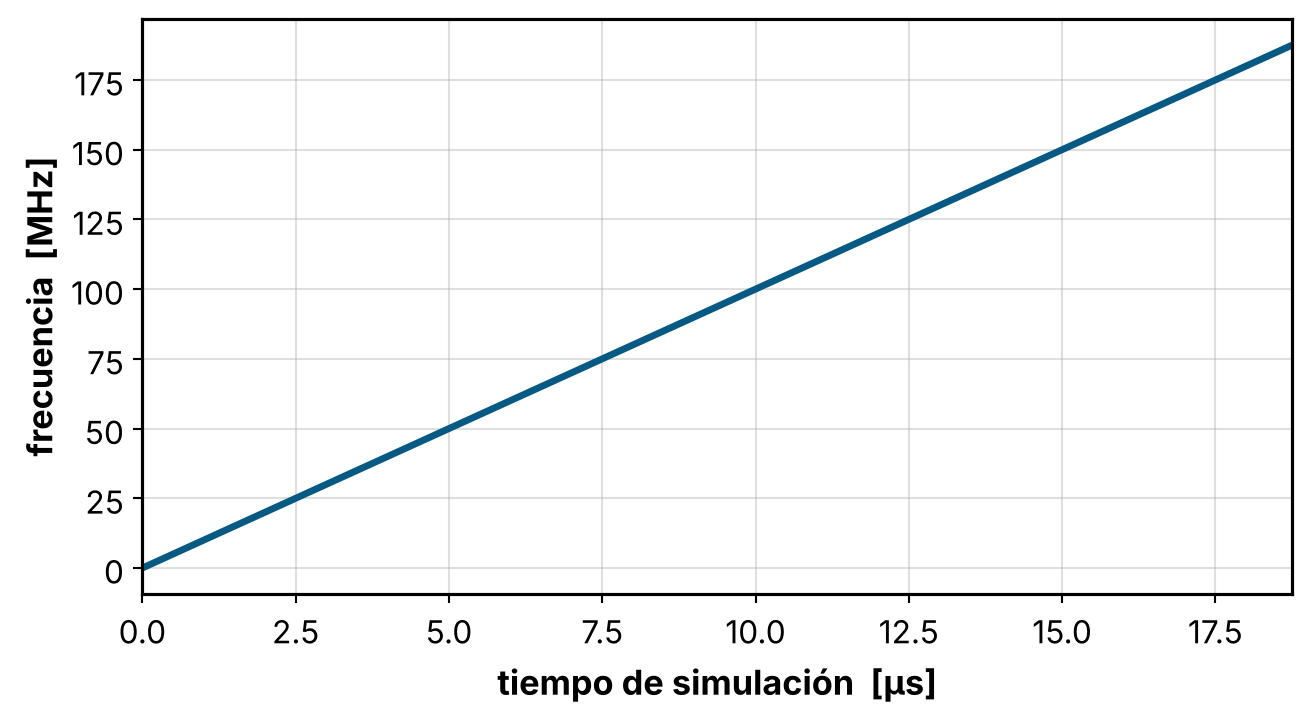
\includegraphics[width=0.78\textwidth]{figuras/rampa_frecuencia_chirp.png}
  \caption[Rampa de frecuencia dejada por el chirp]{%
    Frecuencia instant\'anea a lo largo del registro para un offset inicial
    nulo y una tasa de chirp de \SI{1e13}{\hertz\per\second}.}
  \label{fig:tol-rampa-frecuencia}
\end{figure}

El lazo de recuperaci\'on de fase es de segundo orden, as\'i que ante una
rampa de frecuencia queda con un error de fase estacionario. Ese residuo,
sumado al ruido de fase que aportan el l\'aser transmisor y el oscilador
local, es lo que el lazo tiene que absorber mientras el ecualizador converge.

\begin{figure}[H]
  \centering
  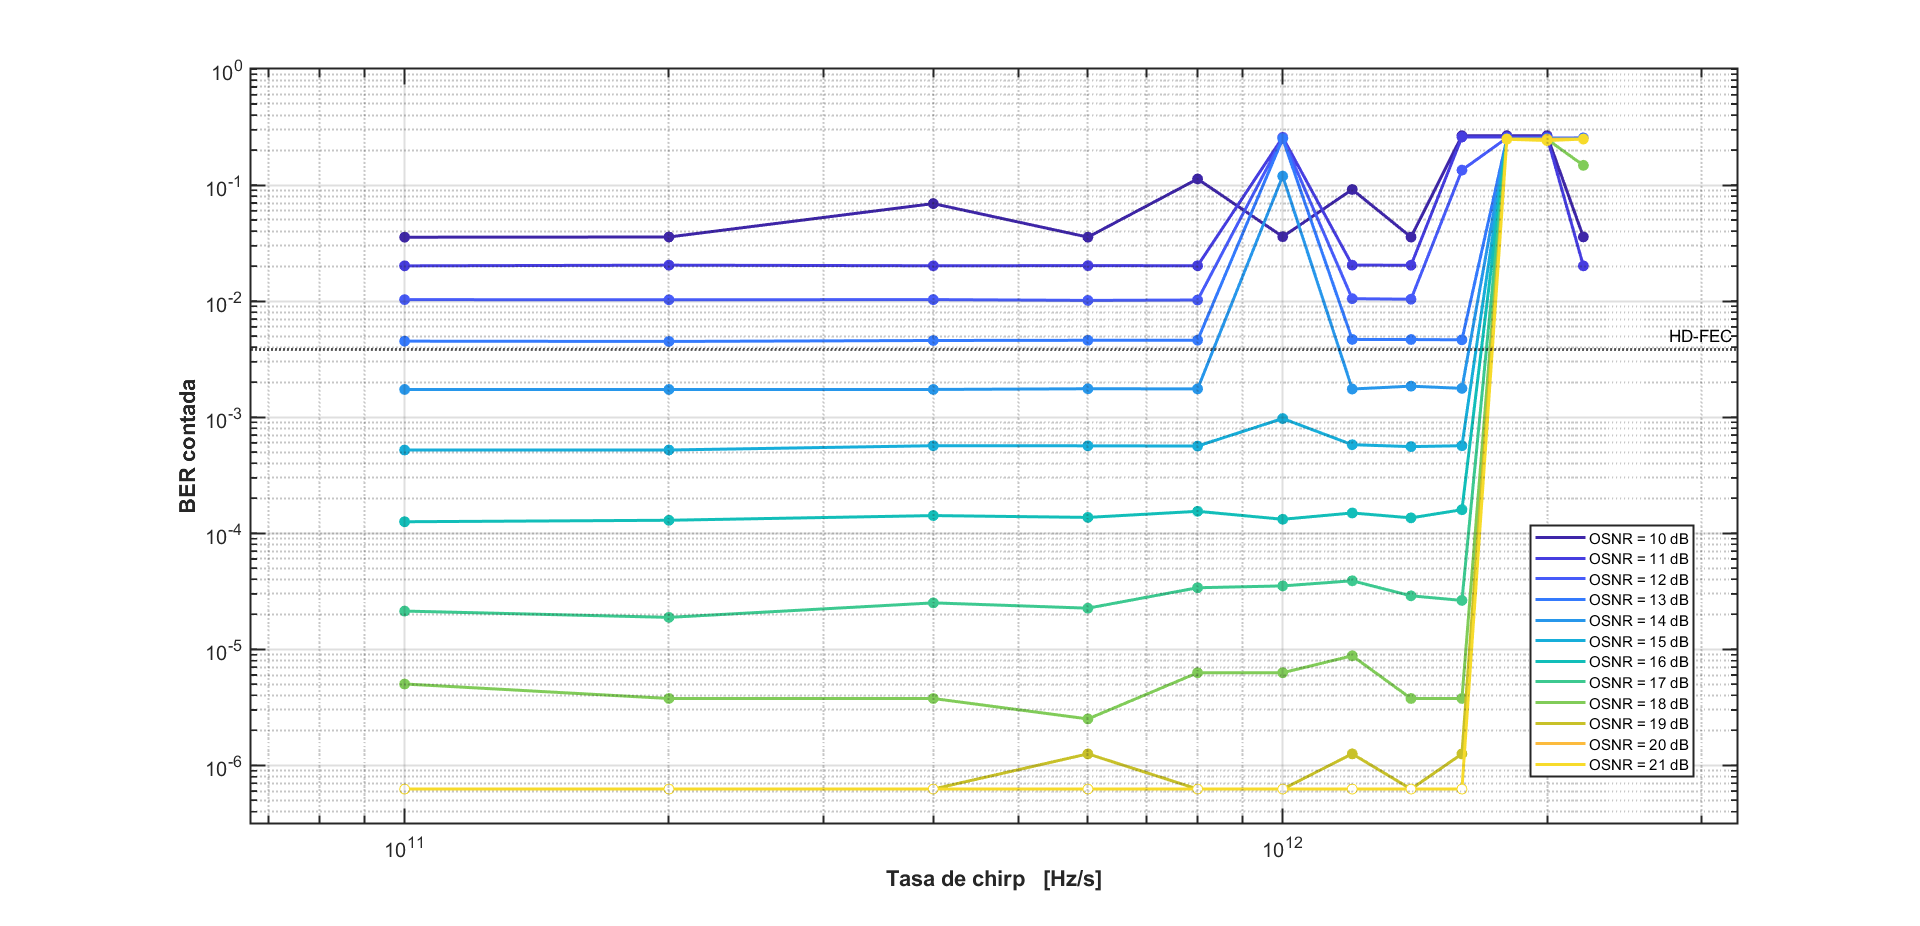
\includegraphics[width=0.92\textwidth]{figuras/tol_chirp_osnr.png}
  \caption[Tolerancia a la tasa de chirp]{%
    BER contra tasa de chirp Doppler para doce valores de OSNR. El color determina la OSNR en pasos de \SI{1}{\dB}, de azul
    oscuro en \SI{10}{\dB} a amarillo en \SI{21}{\dB}. Los c\'irculos huecos
    son puntos sin ning\'un error, dibujados en el piso de conteo. De
    \SI{14}{\dB} en adelante las curvas son planas hasta
    \SI{1.6e12}{\hertz\per\second} y suben hasta \num{0.25} antes de
    \SI{1.8e12}{\hertz\per\second}.}
  \label{fig:tol-chirp}
\end{figure}

La \cref{fig:tol-chirp} barre doce tasas entre \num{1e11} y
\SI{2.2e12}{\hertz\per\second} para doce valores de OSNR. De \SI{14}{\dB} en
adelante la BER se mantiene aproximadamente constante hasta
\SI{1.6e12}{\hertz\per\second} y cruza el umbral HD-FEC entre \num{1.6e12} y
\SI{1.8e12}{\hertz\per\second}, en el mismo intervalo para todas.

El l\'imite no se desplaza con la OSNR. El ruido \'optico no corre el umbral,
pero vuelve a las curvas menos regulares, con fallas aisladas que aparecen en
un punto y desaparecen en el siguiente, como la de
\SI{1e12}{\hertz\per\second} entre \num{11} y \SI{14}{\dB}. Por debajo de
\SI{13}{\dB} las curvas ya arrancan por encima del umbral.

Los resultados sugieren que la falla se asocia a la incapacidad del lazo de
recuperaci\'on de fase para compensar el residuo que deja la variaci\'on
temporal del offset. El quiebre est\'a en \SI{1.8e12}{\hertz\per\second},
m\'as de cinco \'ordenes de magnitud por encima de los
\SI{6.55}{\mega\hertz\per\second} que impone el peor instante del pase, de
modo que el chirp Doppler no representa una limitaci\'on para el enlace.

\section{Rotaci\'on del estado de polarizaci\'on}
\label{sec:tol-sop}

La variaci\'on de la geometr\'ia del enlace LEO--GEO produce una rotaci\'on
din\'amica del estado de polarizaci\'on de la se\~nal recibida, que el
ecualizador MIMO tiene que seguir y compensar. En esta secci\'on se eval\'ua
la capacidad de seguimiento del receptor barriendo la velocidad angular de
rotaci\'on $\dot\theta$ para distintas condiciones de OSNR.

\begin{figure}[H]
  \centering
  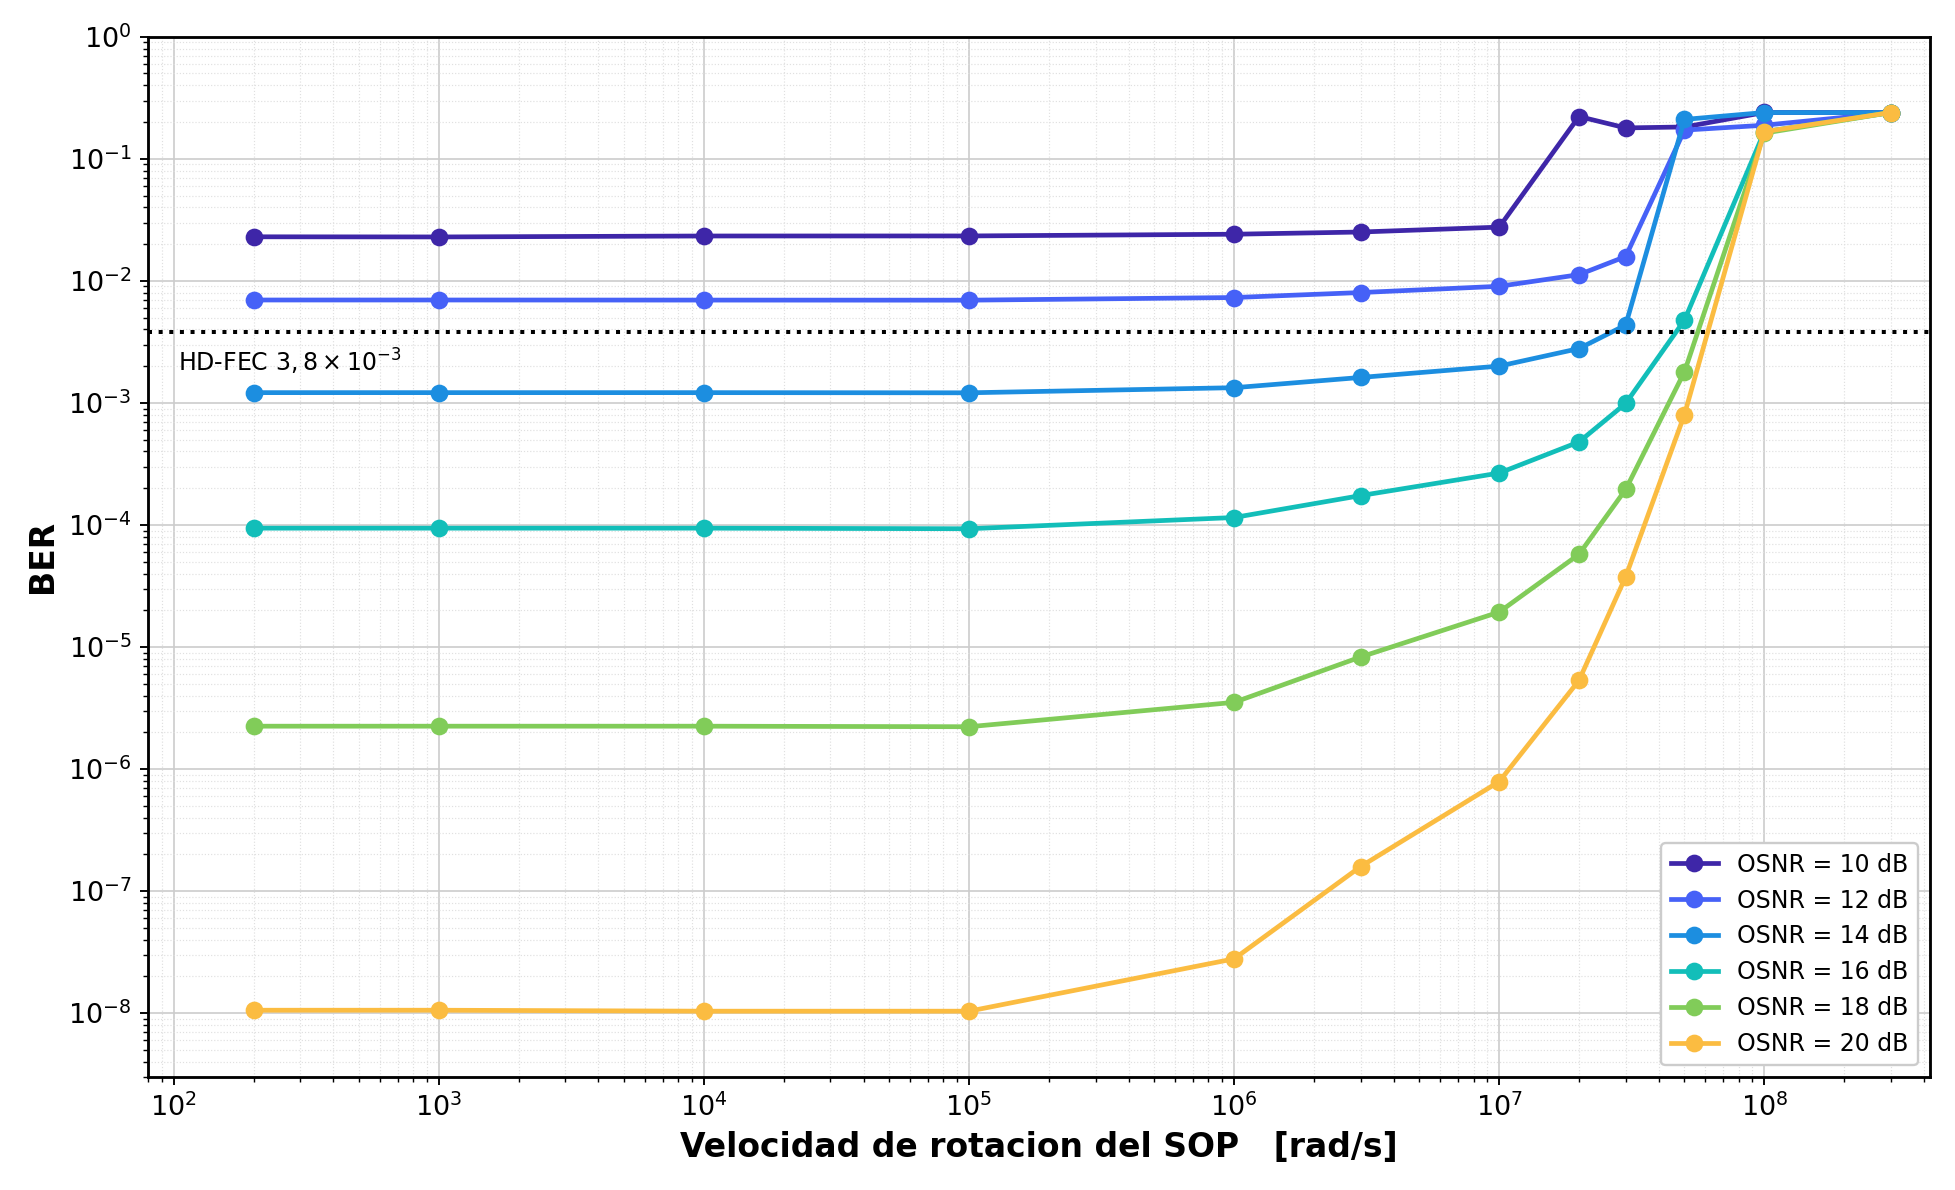
\includegraphics[width=0.92\textwidth]{figuras/SOPOSNR_BER.png}
  \caption[Tolerancia a la rotaci\'on del estado de polarizaci\'on]{%
    BER contra velocidad de rotaci\'on del estado de polarizaci\'on para una
    familia de OSNR. La degradaci\'on empieza a notarse en
    \SI{1e6}{\radian\per\second}, con la primera degradaci\'on pr\'acticamente en el mismo
    lugar para todas las OSNR.}
  \label{fig:tol-sop}
\end{figure}

La capacidad de seguimiento del ecualizador depende de su paso de
adaptaci\'on $\mu$. Un paso mayor actualiza los coeficientes m\'as r\'apido y
reduce el retardo frente a las variaciones del estado de polarizaci\'on.
Tomando una constante de tiempo de adaptaci\'on proporcional a
$1/(\mu\Rs)$~\cite{haykin2014}, el error angular de seguimiento queda, de
forma aproximada,
\begin{equation}
  \theta_{\mathrm{lag}} = \frac{\dot\theta}{\mu \Rs}.
  \label{eq:tol-lag}
\end{equation}
Esta relaci\'on sugiere que, para un error angular m\'aximo tolerable, la
velocidad de rotaci\'on que el ecualizador puede compensar crece en
proporci\'on directa con $\mu$. La \cref{fig:tol-sop-mu} barre doce pasos de
adaptaci\'on y muestra hasta d\'onde vale esa proporcionalidad.

\begin{figure}[H]
  \centering
  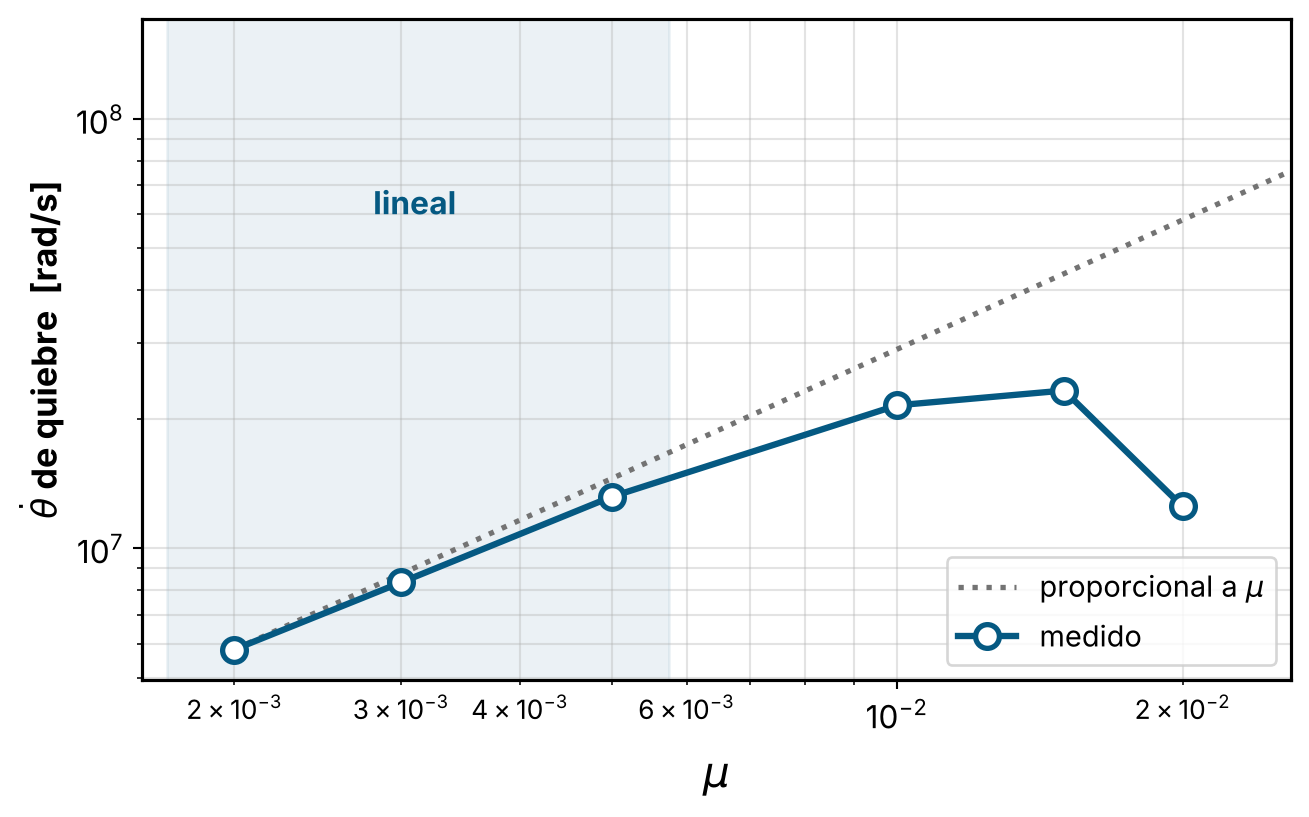
\includegraphics[width=0.82\textwidth]{figuras/tol_quiebre_vs_mu.png}
  \caption[Velocidad de quiebre contra el paso de adaptaci\'on]{%
    Velocidad de rotaci\'on a la que el EVM cruza el umbral HD-FEC, contra el
    paso de adaptaci\'on del ecualizador. La franja marca el tramo en que la
    proporcionalidad con $\mu$ se cumple.}
  \label{fig:tol-sop-mu}
\end{figure}

La proporcionalidad se cumple para los tres pasos m\'as chicos. En
$\mu = \num{0.01}$, que es el valor nominal, el quiebre medido ya se aparta
de la recta, y para valores mayores la tolerancia alcanza un m\'aximo y
despu\'es disminuye.

El comportamiento responde a dos efectos contrapuestos. Un paso mayor permite
seguir variaciones m\'as r\'apidas, pero tambi\'en aumenta el error residual
asociado al ruido de gradiente del ecualizador. El EVM en ausencia de
rotaci\'on sube de \SI{34.4}{\percent} en $\mu = \num{0.002}$ a
\SI{36.6}{\percent} en \num{0.02}, lo que reduce el margen disponible hasta
el umbral HD-FEC. Los dos efectos se compensan alrededor de
$\mu = \num{0.015}$, y por encima de \num{0.025} el receptor deja de cumplir
el requisito de BER incluso con el estado de polarizaci\'on quieto.

Para el paso nominal $\mu = \num{0.01}$ el receptor tolera velocidades de
hasta \SI{2.15e7}{\radian\per\second}, m\'as de diez \'ordenes de magnitud
por encima de los \SI{1e-3}{\radian\per\second} que impone la geometr\'ia del
pase. El estado de polarizaci\'on, por lo tanto, no representa una
limitaci\'on para el enlace.

El modelo de canal incorpora, adem\'as de la deriva geom\'etrica, el jitter
mec\'anico que introduce el control de actitud de la plataforma. Quedan fuera
las variaciones de polarizaci\'on que originan las perturbaciones
mec\'anicas y t\'ermicas sobre los tramos de fibra del transmisor y del
receptor. Dado el margen de diez \'ordenes de magnitud, esos efectos no
cambian la conclusi\'on, pero una implementaci\'on real tiene que
caracterizarlos.

\section{Ruido del l\'aser}
\label{sec:tol-laser}

El ruido de fase del l\'aser transmisor y del oscilador local introduce
fluctuaciones aleatorias en la fase de la se\~nal detectada, que el lazo de
recuperaci\'on de fase tiene que compensar. El par\'ametro barrido en esta
secci\'on es el ancho de l\'inea por l\'aser, $\dnu$. Suponiendo fuentes
independientes con espectro lorentziano, el ancho de l\'inea efectivo del
batido es la suma de los dos.

\subsection{Dependencia con la relaci\'on se\~nal-ruido}
\label{sec:tol-laser-osnr}

\begin{figure}[H]
  \centering
  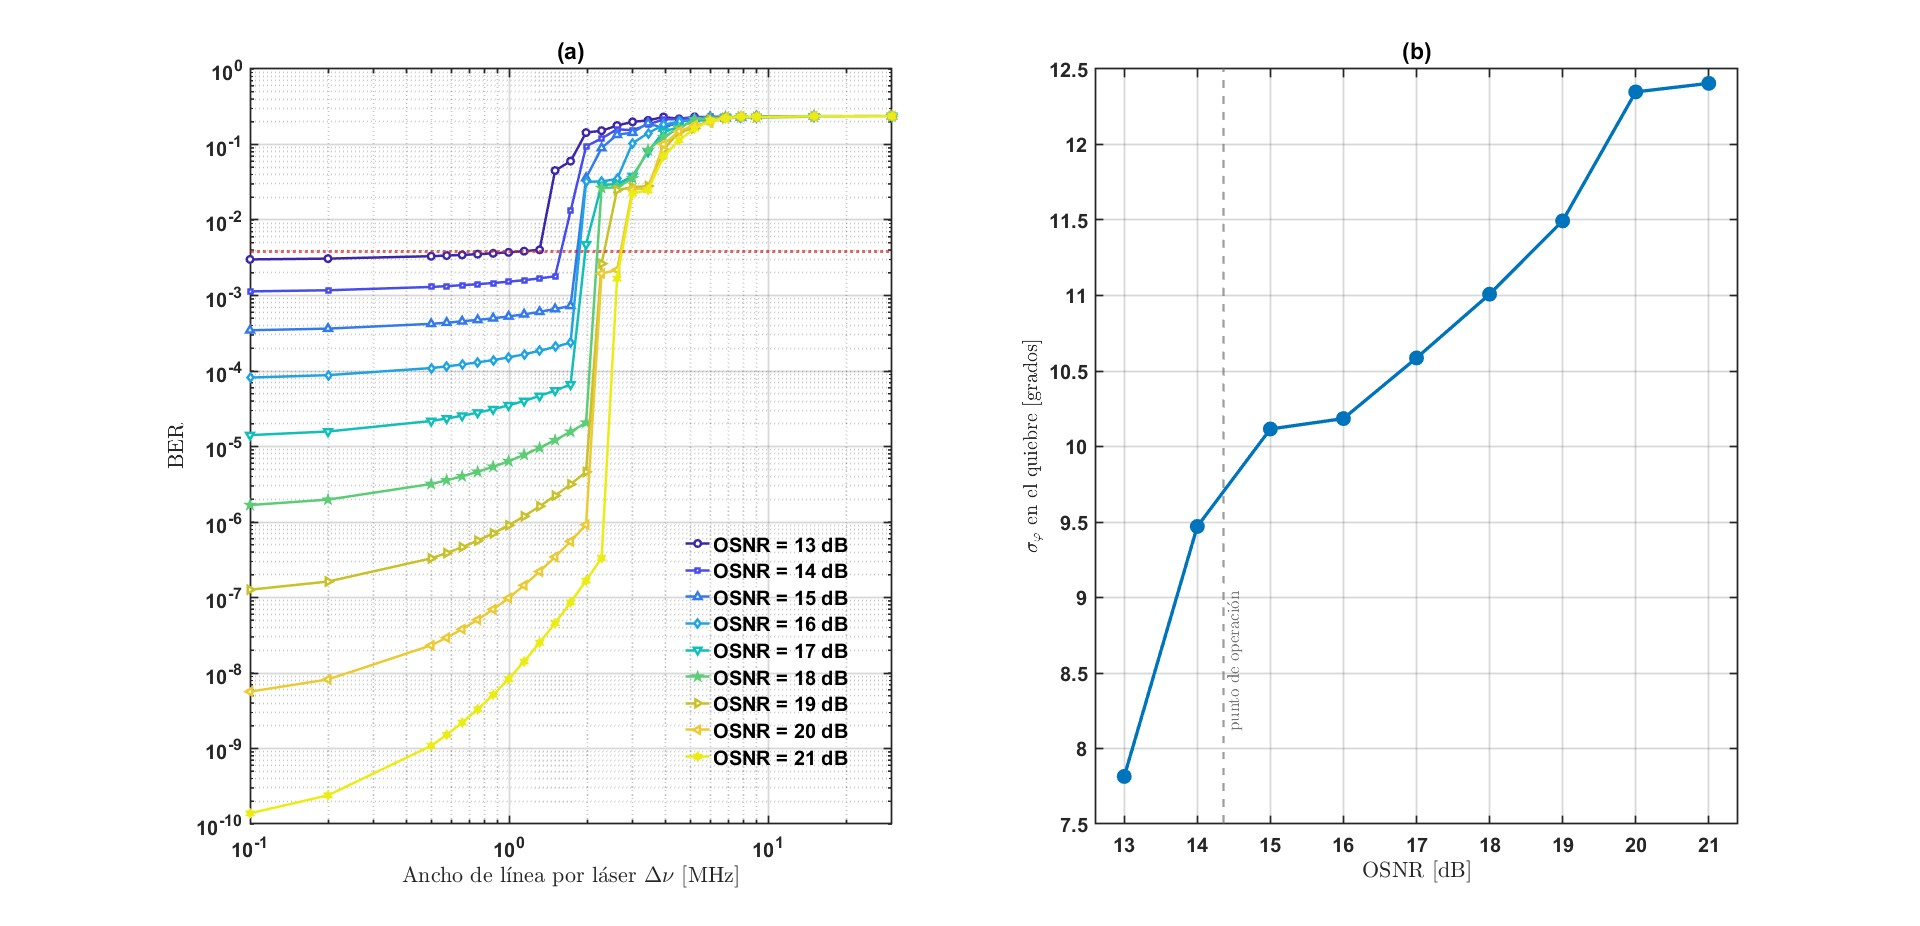
\includegraphics[width=0.98\textwidth]{figuras/TolAnchodeLineaFamiliaOSNR.jpg}
   \caption[Tolerancia al ancho de l\'inea contra OSNR]{%
    (a) BER contra ancho de l\'inea por l\'aser, para una familia de nueve
    valores de OSNR, con $g_1 = \num{0.02}$. El color determina la OSNR en
    pasos de \SI{1}{\dB}, de azul oscuro en \SI{13}{\dB} a amarillo en
    \SI{21}{\dB}. (b) Desviaci\'on est\'andar del error de fase residual,
    evaluada en el quiebre de cada curva. La BER se obtiene del EVM con
    $\mathrm{BER} = Q(1/\EVM)$, que es la misma conversi\'on que define el
    umbral de la \cref{sec:tol-metodologia}.}
  \label{fig:tol-linewidth}
\end{figure}

Como se observa en la \cref{fig:tol-linewidth}a, el aumento del ancho de
l\'inea degrada el desempe\~no de forma gradual. La BER sube de manera
continua y cada curva cruza el umbral en un punto propio. Ese punto mejora
con la OSNR, de \SI{1.6}{\mega\hertz} por l\'aser en \SI{14}{\dB} a
\SI{2.7}{\mega\hertz} en \SI{21}{\dB}.

El panel (b) muestra que la desviaci\'on del error de fase en el quiebre
tampoco es constante. Crece un \SI{59}{\percent} entre \SI{13}{\dB} y
\SI{21}{\dB}. Con menos ASE queda m\'as EVM disponible antes del umbral, de
modo que el lazo tolera excursiones de fase mayores. El l\'imite de
tolerancia al ruido de fase depende entonces de la OSNR de operaci\'on. Esto
no invalida la ley de escala de la \cref{sec:tol-laser-ley}, que se verifica
a OSNR fija, pero s\'i obliga a reportar su constante atada al punto de
operaci\'on.

\subsection{Verificaci\'on de la ley de escala}
\label{sec:tol-laser-ley}

La \cref{eq:var-fase} predice que el quiebre ocurre siempre a la misma
desviaci\'on de fase residual, cualquiera sea la combinaci\'on de ancho de
l\'inea y ancho de banda de lazo. Se puso a prueba esta afirmaci\'on al barrer la
ganancia del lazo y verificar si todas las curvas colapsan en el mismo punto.

\begin{figure}[H]
  \centering
  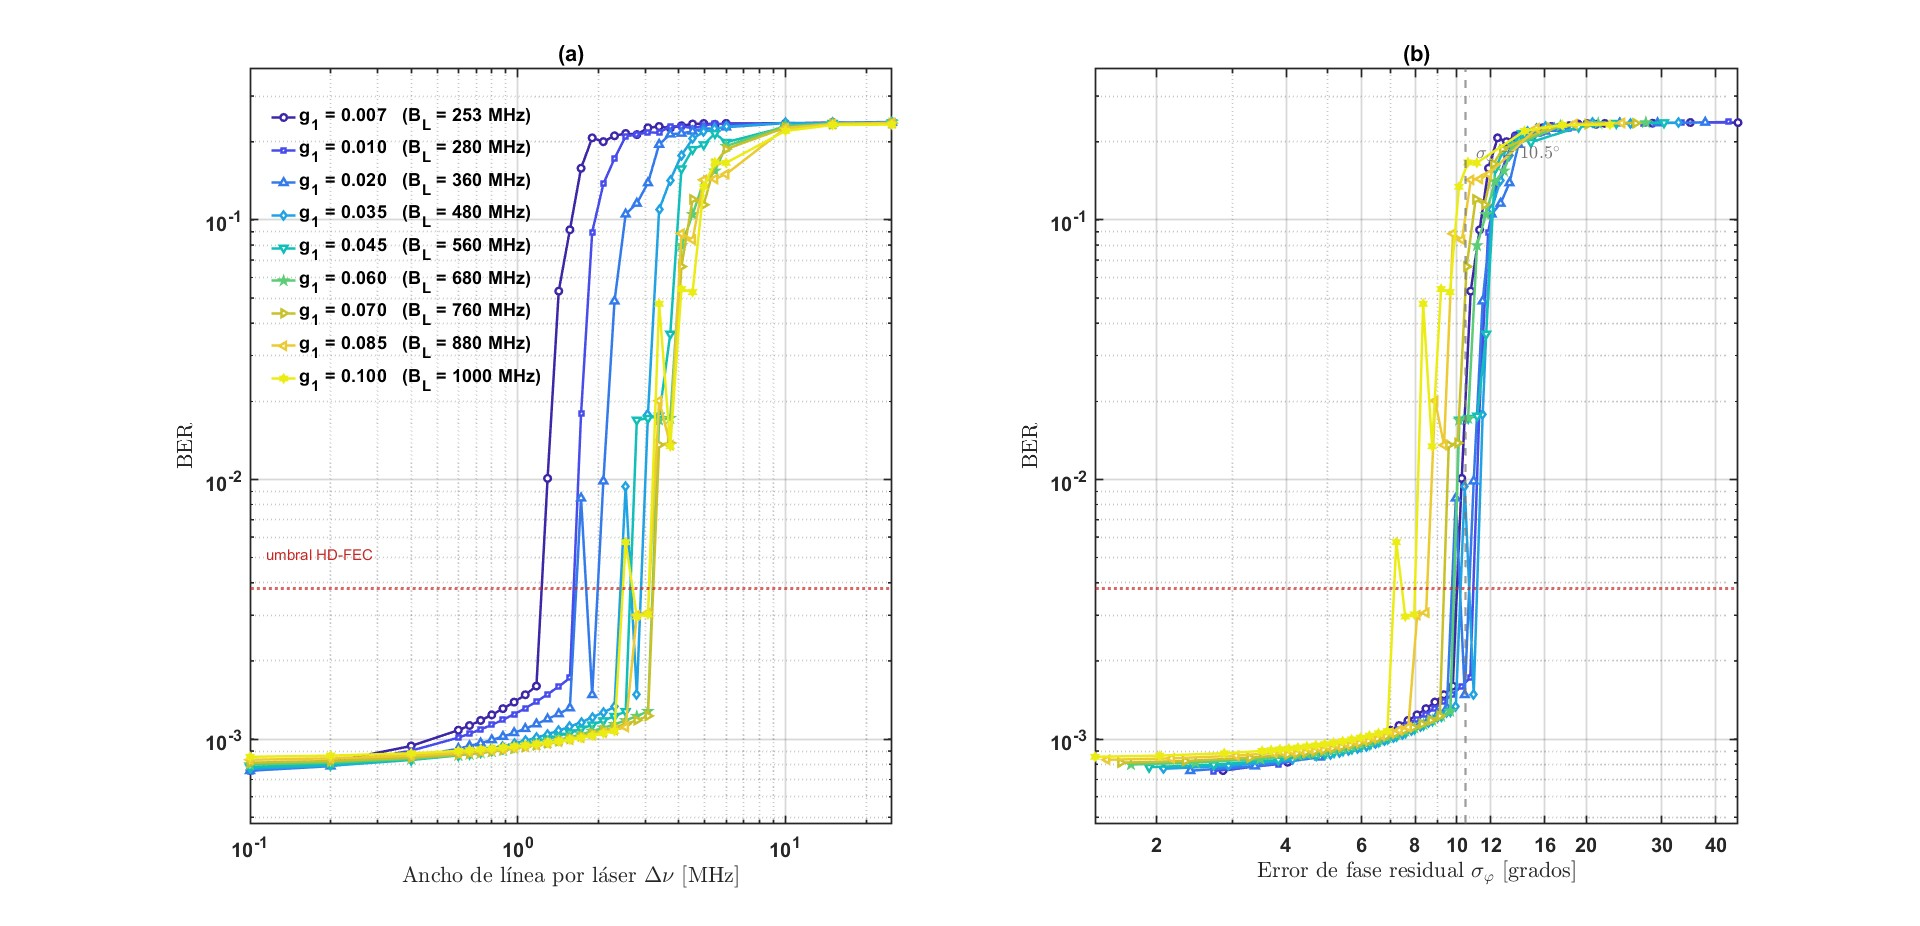
\includegraphics[width=0.98\textwidth]{figuras/TolAnchoLineaLey.jpg}
  \caption[Verificaci\'on de la ley de ruido de fase]{%
    (a) BER contra ancho de l\'inea por l\'aser, una curva por cada valor de
    $g_1$, a $\OSNR = \SI{14.4}{\dB}$. (b) Las mismas curvas contra el error
    de fase residual de la \cref{eq:var-fase}. Si la ley vale, todas tienen
    que cruzar el umbral en el mismo punto del eje horizontal.}
  \label{fig:tol-ley}
\end{figure}

El colapso se verifica sobre las seis curvas de menor ganancia, con
$\sigma_\varphi = \ang{10.5}$ y una dispersi\'on del \SI{5}{\percent}.

Este valor se interpreta contra el margen angular de QPSK, que es de
$\pm\ang{45}$. El cociente entre los dos vale
\begin{equation}
  \frac{\ang{45}}{\sigma_\varphi} = \num{4.3},
  \label{eq:cuatro-sigma}
\end{equation}
es decir que el receptor falla justo donde la cola de la distribuci\'on de
fase empieza a cruzar la frontera de decisi\'on con probabilidad apreciable.
Como muestra la \cref{sec:tol-laser-osnr}, ese cociente no es universal,
porque depende de la OSNR.

\begin{table}[htbp]
  \centering
  \begin{tabular}{lccc}
    \toprule
    $g_1$ & $B_L$ & $\dnu$ de quiebre [\si{\mega\hertz}] & $\sigma_\varphi$ \\
    \midrule
    \num{0.0067} & \SI{253}{\mega\hertz}  & \num{1.22} & \ang{9.96}  \\
    \num{0.010}  & \SI{280}{\mega\hertz}  & \num{1.60} & \ang{10.87} \\
    \num{0.020}  & \SI{360}{\mega\hertz}  & \num{1.97} & \ang{10.63} \\
    \num{0.035}  & \SI{480}{\mega\hertz}  & \num{2.86} & \ang{11.08} \\
    \num{0.045}  & \SI{560}{\mega\hertz}  & \num{2.61} & \ang{9.80}  \\
    \num{0.060}  & \SI{680}{\mega\hertz}  & \num{3.16} & \ang{9.79}  \\
    \midrule
    \num{0.070}  & \SI{760}{\mega\hertz}  & \num{3.17} & \ang{9.28}  \\
    \num{0.085}  & \SI{880}{\mega\hertz}  & \num{3.09} & \ang{8.51}  \\
    \num{0.100}  & \SI{1000}{\mega\hertz} & \num{3.08} & \ang{7.97}  \\
    \bottomrule
  \end{tabular}
  \caption[Ancho de l\'inea de quiebre contra la ganancia del lazo]{%
    Ancho de l\'inea de quiebre y desviaci\'on de fase residual que resulta,
    a $\OSNR = \SI{14.4}{\dB}$. Las seis primeras filas son las que cumplen
    la ley. Las \'ultimas tres se apartan, con un quiebre que deja de
    crecer y un $\sigma_\varphi$ que baja de forma monot\'ona.}
  \label{tab:tol-linewidth}
\end{table}

La \cref{tab:tol-linewidth} recorre las nueve ganancias ensayadas, con el
ancho de l\'inea de quiebre que resulta en cada una. La elecci\'on de la
ganancia de operaci\'on se discute en la \cref{sec:tol-laser-diseno}.

\subsection{Alcance y punto de dise\~no}
\label{sec:tol-laser-diseno}

Las \'ultimas tres filas de la \cref{tab:tol-linewidth} se apartan de la
ley. El quiebre se queda en unos \SI{3.1}{\mega\hertz} aunque el ancho de
banda del lazo siga creciendo.

\begin{figure}[H]
  \centering
  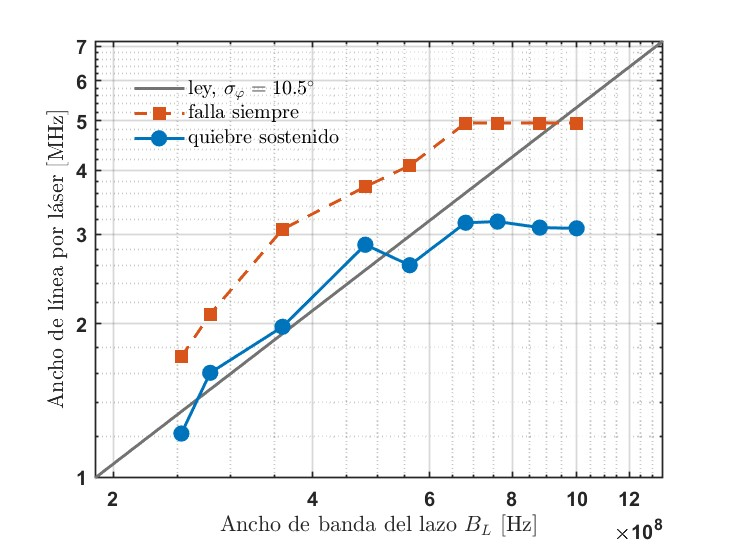
\includegraphics[width=0.72\textwidth]{figuras/TolAnchoLineaDiseno.jpg}
  \caption[Alcance de la ley de escala]{%
    Ancho de l\'inea de quiebre contra ancho de banda del lazo, con la recta
    de la ley ajustada sobre las curvas que la cumplen. Se agrega el ancho de
    l\'inea a partir del cual fallan todas las semillas. Entre las dos curvas
    se encuentra la banda en la que el receptor funciona o no seg\'un la
    realizaci\'on del ruido.}
  \label{fig:tol-diseno}
\end{figure}

La separaci\'on entre las dos curvas de la \cref{fig:tol-diseno} es la zona de
transici\'on. La falla no es una degradaci\'on sino un deslizamiento de ciclo, o cycle slip,
de modo que no hay un umbral duro sino una probabilidad creciente. Con
$g_1 = \num{0.02}$ el receptor empieza a fallar de forma aislada en
\SI{1.97}{\mega\hertz} y falla siempre a partir de \SI{3.07}{\mega\hertz}.

En la \cref{fig:tol-dosg1} se analizan dos valores de ganancia, con sus puntos de quiebre para una familia de OSNR.

\begin{figure}[H]
  \centering
  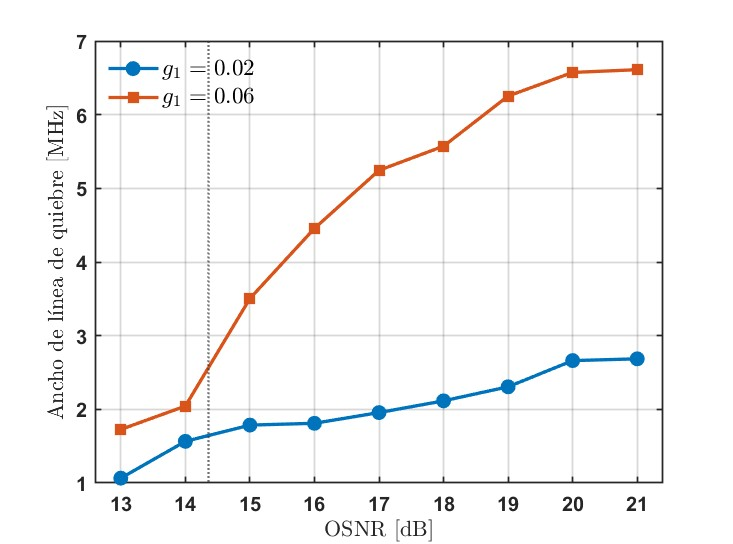
\includegraphics[width=0.72\textwidth]{figuras/TolAnchodeLineaDosValG1.jpg}
  \caption[Quiebre contra OSNR para dos ganancias de lazo]{%
    Ancho de l\'inea de quiebre contra OSNR, para dos valores de ganancia. Las dos curvas crecen con la OSNR y
    la del lazo ancho crece m\'as r\'apido.}
  \label{fig:tol-dosg1}
\end{figure}

Entre \SI{13}{\dB} y \SI{21}{\dB} el quiebre de $g_1 = \num{0.02}$ mejora un
factor \num{2.5}, mientras que el de $g_1 = \num{0.06}$ mejora un factor
\num{3.8}. El lazo ancho se beneficia m\'as de bajar el ASE. Esto indica que lo
que lo limita a OSNR baja es el ruido aditivo que integra, y no un l\'imite
propio del lazo. Si fuese as\'i, el quiebre de
$g_1 = \num{0.06}$ se habr\'ia mantenido constante al mejorar la OSNR. A 
OSNR alta la mejora es cada vez menor por \si{\dB} de OSNR. En este caso el factor de falla predominante es el l\'imite propio del lazo, es decir, su ancho de banda, en lugar del ruido aditivo.

Se concluye que pasar de \num{0.02} a \num{0.06} sube la tolerancia un factor
\num{1.6}, en lugar del \num{1.9} que predice el ajuste de la
\cref{fig:tol-diseno}.

Con esto queda fijado el punto de dise\~no. La ganancia del lazo de fase se
fij\'o en $g_1 = \num{0.06}$, que por las expresiones de la
\cref{sec:dsp-cpr} corresponde a $B_L = \SI{680}{\mega\hertz}$ y a un
amortiguamiento de $\zeta = \num{0.77}$. 

Hacia valores menores de $B_L$, la tolerancia se pierde en proporci\'on con \'el, tal como
predice la \cref{eq:var-fase}. Hacia valores mayores, y a OSNR constante, satura porque el lazo pasa a
integrar m\'as ruido aditivo del que gana en seguimiento de la fase. Con esta
ganancia el receptor tolera \SI{3.16}{\mega\hertz} de ancho de l\'inea por
l\'aser, de modo que contra el requisito de \SI{100}{\kilo\hertz} el margen es
de un factor \num{32}. El l\'aser del laboratorio, de \SI{15}{\kilo\hertz},
est\'a un factor \num{210} por debajo del quiebre.

\subsection{Ruido de intensidad relativa}
\label{sec:tol-rin}

El ruido de intensidad se barri\'o con la misma familia de OSNR, como se ve en la \cref{fig:tol-rin}. La respuesta es plana desde
\SI{-165}{\dB\per\hertz} hasta \SI{-140}{\dB\per\hertz}, que es el valor de los l\'aseres
utilizados, y el desempe\~no empieza a degradarse reci\'en en
\SI{-130}{\dB\per\hertz}. El cruce del umbral va de \SI{-120}{\dB\per\hertz}
en \SI{13}{\dB} de OSNR a \SI{-109}{\dB\per\hertz} desde \SI{17}{\dB} en
adelante.


\begin{figure}[H]
  \centering
  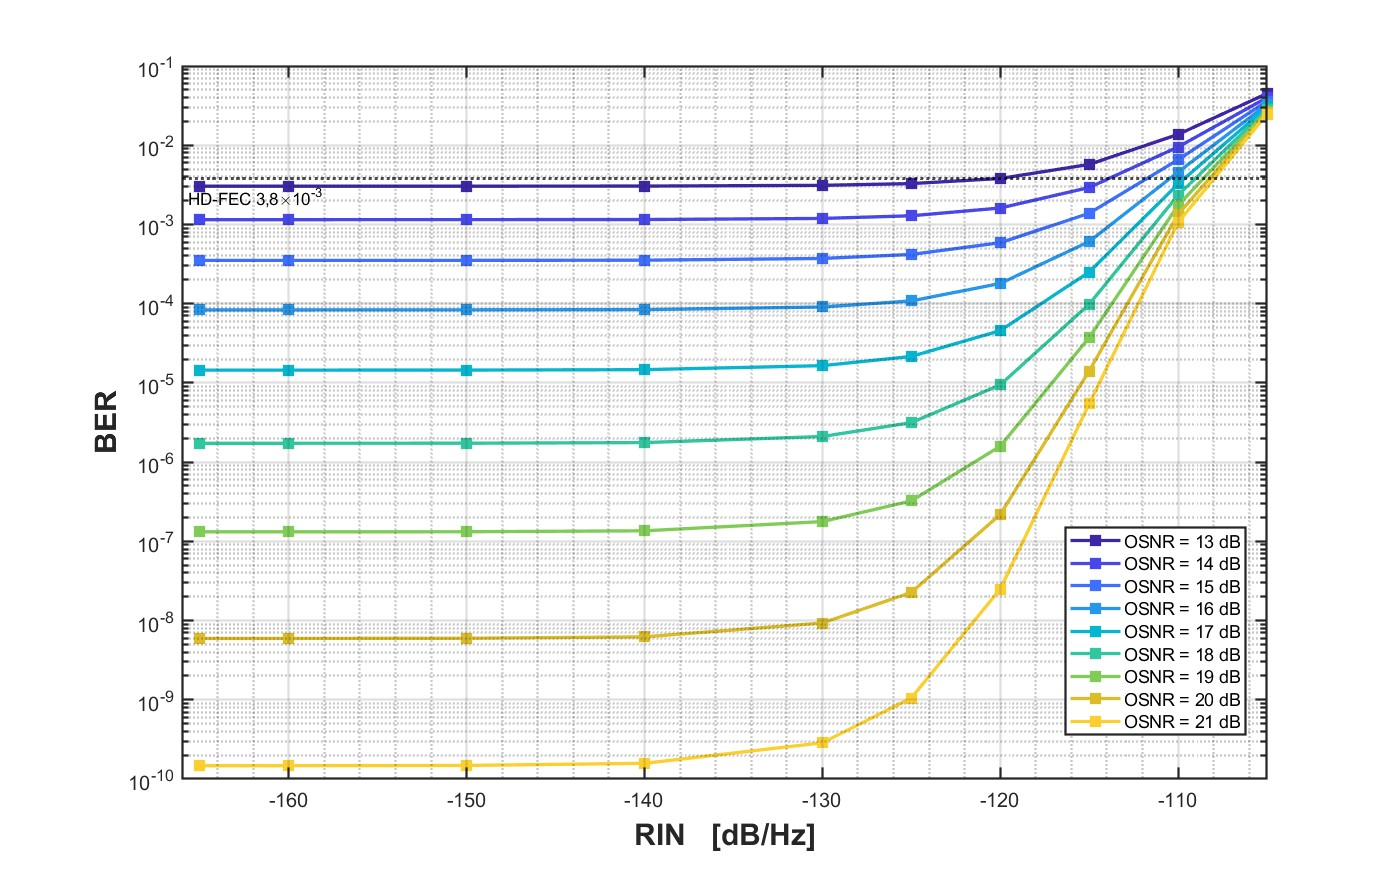
\includegraphics[width=0.92\textwidth]{figuras/BarridoRINOSNR.jpg}
  \caption[Tolerancia al RIN]{%
    BER en funci\'on del RIN del l\'aser, para una familia de
    nueve valores de OSNR. El color determina la OSNR en pasos de \SI{1}{\dB}, de azul oscuro en \SI{13}{\dB} a amarillo en \SI{21}{\dB}.}
  \label{fig:tol-rin}
\end{figure}

El RIN degrada el desempe\~no de forma gradual, con un l\'imite que mejora al
bajar el ASE y se aplana por encima de \SI{17}{\dB}. El margen contra el
componente real es amplio en todo el rango simulado.

\section{Deterioros del front end del receptor}
\label{sec:tol-frontend}

En esta secci\'on se analizan los deterioros provenientes del
receptor para encontrar sus tolerancias m\'aximas.

\paragraph{Skew entre las ramas}
El skew es la diferencia de retardo entre los cuatro carriles del front end, y
es el \'unico deterioro de este cap\'itulo cuyo margen es estrecho. Con el
estimador de frecuencia desactivado el ecualizador lo absorbe hasta
\SI{62.5}{\pico\second}. Pero con el estimador de frecuencia activo, que es la condici\'on
real de operaci\'on, la tolerancia cae a \SI{4.5}{\pico\second} para
\SI{0.5}{\dB} de penalidad.

Esto es debido al orden en que est\'an los bloques. Un retardo $\tau$ entre la rama en
fase y la de cuadratura es una operaci\'on ampliamente lineal sobre la se\~nal
compleja: si $x$ es la se\~nal sin deteriorar, la que llega al conversor es
\begin{equation}
  r = A(f)\,x + B(f)\,x^{*},
  \qquad
  \left|\frac{B(f)}{A(f)}\right| = \left|\tan(\pi f \tau)\right|,
  \label{eq:tol-skew-wl}
\end{equation}
con una r\'eplica conjugada que crece hacia los bordes de la banda. El
ecualizador mariposa de este receptor es de filtros reales y espaciado $T/2$,
de modo que tiene los grados de libertad para cancelar la r\'eplica. Es decir, puede
aplicar retardos distintos a la componente en fase y a la de cuadratura, lo que ocurre con el
estimador desactivado, llegando a \SI{62.5}{\pico\second} de tolerancia.

La compensaci\'on de frecuencia multiplica la se\~nal por $e^{-j\omega t}$.
Sin embargo, sobre la r\'eplica
conjugada deja un factor $e^{-j2\omega t}$. El efecto neto es que deja de estar en la frecuencia espejo y pasa a girar a $2\Delta f$ respecto de la se\~nal. Es un deterioro que se vuelve irreversible, porque la cancelaci\'on exige que los coeficientes del ecualizador se adapten a esa velocidad.

\begin{table}[htbp]
  \centering

  \begin{tabular}{lcccc}
    \toprule
    & \multicolumn{4}{c}{Skew entre ramas} \\
    \cmidrule(l){2-5}
    & \SI{0}{\pico\second} & \SI{2}{\pico\second} & \SI{5}{\pico\second}
    & \SI{10}{\pico\second} \\
    \midrule
    $\Df = 0$                      & 35,10 & 35,09 & 35,10 & 35,12 \\
    \midrule
    $\Df = \SI{0.02}{\giga\hertz}$ & 35,10 & 35,31 & 36,66 & colapsa \\
    $\Df = \SI{0.2}{\giga\hertz}$  & 35,10 & 35,47 & 37,44 & colapsa \\
    $\Df = \SI{1}{\giga\hertz}$    & 35,10 & 35,48 & 37,46 & colapsa \\
    $\Df = \SI{2}{\giga\hertz}$    & 35,10 & 35,46 & 37,32 & colapsa \\
    $\Df = \SI{4}{\giga\hertz}$    & 35,10 & 35,39 & 36,93 & colapsa \\
    \bottomrule
  \end{tabular}
  \caption[Origen del l\'imite de skew]{%
    EVM de la peor polarizaci\'on contra skew entre las ramas en fase y
    cuadratura, con el estimador de frecuencia activo, para seis valores de
    offset, a $\OSNR = \SI{14.4}{\dB}$. En la primera fila el offset es nulo y el ecualizador absorbe el
    skew en todo el rango barrido.}
  \label{tab:tol-skew}
\end{table}

La \cref{tab:tol-skew} muestra un an\'alisis de los dos efectos mencionados. Entre
\SI{0.2}{\giga\hertz} y \SI{4}{\giga\hertz} el
colapso sigue cayendo en \SI{10}{\pico\second} y el EVM en
\SI{5}{\pico\second} se mantiene aproximadamente constante. Esto significa que, desde offsets de 
frecuencia peque\~nos como \SI{20}{\mega\hertz}, los coeficientes del ecualizador no llegan a adaptarse, es decir, la penalidad satura desde el principio. Con offset nulo no se tiene una componente espuria rotando, y el ecualizador absorbe el skew hasta los \SI{62.5}{\pico\second} del barrido, al igual que con el bloque desactivado.


El problema, entonces, no es de grados de libertad sino de orden. Una forma de
resolverlo es compensar el skew y el desbalance de cuadratura antes del
recuperador de frecuencia, con una estructura ampliamente lineal
dedicada~\cite{portodasilva2016}, en el punto de la cadena donde la r\'eplica
conjugada todav\'ia est\'a quieta. Esto implicar\'ia reordenar la cadena del
DSP y rehacer los an\'alisis correspondientes.

Con la cadena actual, es necesario hacer una calibraci\'on del front end receptor antes de entrar en operaci\'on. El skew tiene que quedar por debajo de
\SI{4.5}{\pico\second} para tener una penalidad menor a \SI{0.5}{\dB}.


\paragraph{Error de reloj}
El desajuste entre el reloj del transmisor y el del ADC del receptor se tolera
hasta \SI{175}{\ppm}. El l\'imite lo impone el rango de enganche del lazo de
segundo orden, no la longitud de la secuencia de s\'imbolos. Un desajuste de reloj mueve el
instante de muestreo un poco por s\'imbolo, siempre en el mismo sentido, de
modo que el corrimiento se acumula a lo largo de la simulaci\'on. A
\SI{175}{\ppm} ese corrimiento pasa de \num{8.8} per\'iodos de s\'imbolo en una
secuencia de \num{5e4} a \num{70} en uno de \num{4e5}. Repitiendo el barrido en
todo ese rango el punto de falla no se mueve, lo que descarta al corrimiento
acumulado como causa. Contra los \SI{25.55}{\ppm} que impone el Doppler sobre
la tasa de s\'imbolos, el margen es de un factor \num{6.8}, y deja unos
\SI{150}{\ppm} de presupuesto para la deriva del oscilador del receptor.

\paragraph{Fase de muestreo, error de cuadratura y desbalance de ganancia}
Ninguno de los tres impone l\'imite en el rango explorado. El desajuste de fase
de muestreo se barri\'o hasta $1{,}0\,\Ts$, es decir un s\'imbolo completo,
sin penalidad medible.
El error de cuadratura del h\'ibrido se barri\'o hasta \SI{18}{\degree} con el
mismo resultado, porque la ortogonalizaci\'on de Gram-Schmidt lo invierte de
forma exacta, seg\'un se mostr\'o en la \cref{sec:dsp-gsop}.
El desbalance de ganancia entre las ramas tiene un resultado similar. Se barri\'o
hasta un cociente de \num{0.30}, es decir un factor tres entre las dos
ramas, sin penalidad medible.


\section{Presupuesto conjunto de deterioros}
\label{sec:tol-presupuesto}

En las secciones anteriores se midi\'o cada deterioro por separado. Esta secci\'on analiza diferentes casos con distintas configuraciones de deterioros, a trav\'es de un barrido sobre nueve valores de OSNR.

Se midieron trece configuraciones, numeradas de \Cfg{0} a \Cfg{12} y definidas
en la \cref{tab:tol-configs}. Todas comparten el mismo punto de partida, que es
el receptor con el l\'aser nominal de \SI{100}{\kilo\hertz} y el offset
Doppler de \SI{2}{\giga\hertz} que usa todo el cap\'itulo, y se distinguen por
lo que se agrega encima.

\Cfg{0} es ese punto de partida sin nada agregado y sirve de referencia para
todos los dem\'as casos. De \Cfg{1} a \Cfg{3} se activa un deterioro por vez, con
niveles calibrados de antemano para que los tres cuesten lo mismo por separado:
ancho de l\'inea de \SI{1.333}{\mega\hertz}, deriva de polarizaci\'on de
\SI{14.53}{\mega\radian\per\second} y skew de \SI{3.789}{\pico\second}. De
\Cfg{4} a \Cfg{7} se combinan esos mismos tres niveles de a pares y de a
tres.

Por otro lado, los cinco \'ultimos casos usan los valores de especificaci\'on del
enlace.
\Cfg{8} agrega los dos deterioros que var\'ian a lo largo del pase, la deriva
de polarizaci\'on y el error de cuadratura del h\'ibrido. \Cfg{9} agrega los
cuatro que son valores fijos de especificaci\'on, el Doppler, el error de
reloj, el desajuste de fase de muestreo y el skew. \Cfg{10} tiene todos los deterioros a
la vez, mostrando el peor caso de vuelo. \Cfg{11} y \Cfg{12} repiten \Cfg{10} con el
skew calibrado a \SI{2}{\pico\second} y \SI{0}{\pico\second}.

\begin{table}[htbp]
  \centering
  \small
  \setlength{\tabcolsep}{4.5pt}

  \begin{tabular}{llccccccc}
    \toprule
    & & $\dnu$ & SOP & $\varphi$ & $\Df$ & reloj & fase & skew \\
    & & [\si{\kilo\hertz}] & [\si{\radian\per\second}] & [\si{\degree}]
      & [\si{\giga\hertz}] & [\si{\ppm}] & [$\Ts$] & [\si{\pico\second}] \\
    \midrule
    \Cfg{0}    & referencia        & ---  & ---        & --- & --- & ---   & ---  & ---  \\
    \midrule
    \Cfg{1}    & \multirow{7}{*}{\parbox{2.6cm}{niveles\\calibrados}}
                                   & 1333 & ---        & --- & --- & ---   & ---  & ---  \\
    \Cfg{2}    & & ---  & \num{1.453e7} & --- & --- & ---   & ---  & ---  \\
    \Cfg{3}   & & ---  & ---          & --- & --- & ---   & ---  & 3,79 \\
    \Cfg{4} & & 1333 & \num{1.453e7} & --- & --- & ---   & ---  & ---  \\
    \Cfg{5}  & & 1333 & ---          & --- & --- & ---   & ---  & 3,79 \\
    \Cfg{6}   & & ---  & \num{1.453e7} & --- & --- & ---   & ---  & 3,79 \\
    \Cfg{7}  & & 1333 & \num{1.453e7} & --- & --- & ---   & ---  & 3,79 \\
    \midrule
    \Cfg{8}   & \multirow{5}{*}{\parbox{2.6cm}{valores\\de vuelo}}
                                   & ---  & \num{e-3}  & 3   & --- & ---   & ---  & ---  \\
    \Cfg{9}  & & ---  & ---        & --- & 6   & 25,55 & 0,25 & 5    \\
    \Cfg{10}   & & ---  & \num{e-3}  & 3   & 6   & 25,55 & 0,25 & 5    \\
    \Cfg{11}   & & ---  & \num{e-3}  & 3   & 6   & 25,55 & 0,25 & 2    \\
    \Cfg{12}   & & ---  & \num{e-3}  & 3   & 6   & 25,55 & 0,25 & ---  \\
    \bottomrule
  \end{tabular}
  \caption[Configuraciones de deterioros del presupuesto]{%
    Las trece configuraciones del presupuesto. Un gui\'on indica que el
        deterioro est\'a en su valor neutro, es decir ausente, salvo en las
    columnas de $\dnu$ y $\Df$, donde significa que se mantiene el valor
    base de todo el cap\'itulo, \SI{100}{\kilo\hertz} de ancho de l\'inea por
    l\'aser y \SI{2}{\giga\hertz} de offset Doppler.}
  \label{tab:tol-configs}
\end{table}

\begin{figure}[H]
  \centering
  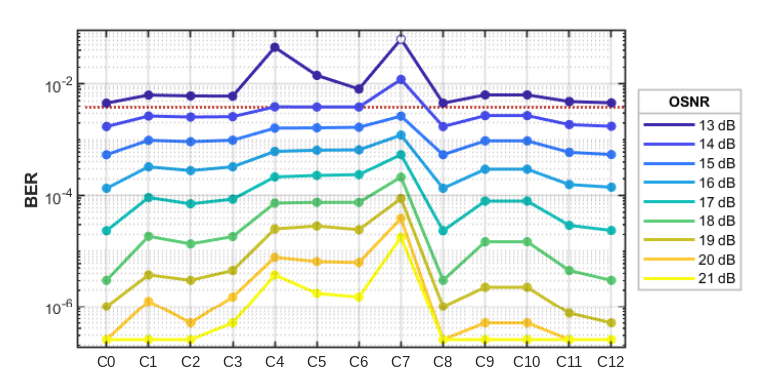
\includegraphics[width=0.95\textwidth]{figuras/tol_ber_vs_deterioro.png}
  \caption[BER de cada configuraci\'on de deterioros]{%
    BER de las trece configuraciones de la \cref{tab:tol-configs} para la
    familia de OSNR simuladas, de \SIrange{13}{21}{\dB}. El color determina la
    OSNR, de azul oscuro en \SI{13}{\dB} a amarillo en \SI{21}{\dB}.}
  \label{fig:tol-familia}
\end{figure}

La \cref{fig:tol-familia} pone las trece configuraciones una al lado de la
otra para las nueve OSNR de \SIrange{13}{21}{\dB}. El orden entre ellas es el
mismo en el resto de figuras, as\'i que alcanza con resumir cada configuraci\'on por la OSNR
a la que cruza el umbral HD-FEC.

\begin{figure}[H]
  \centering
  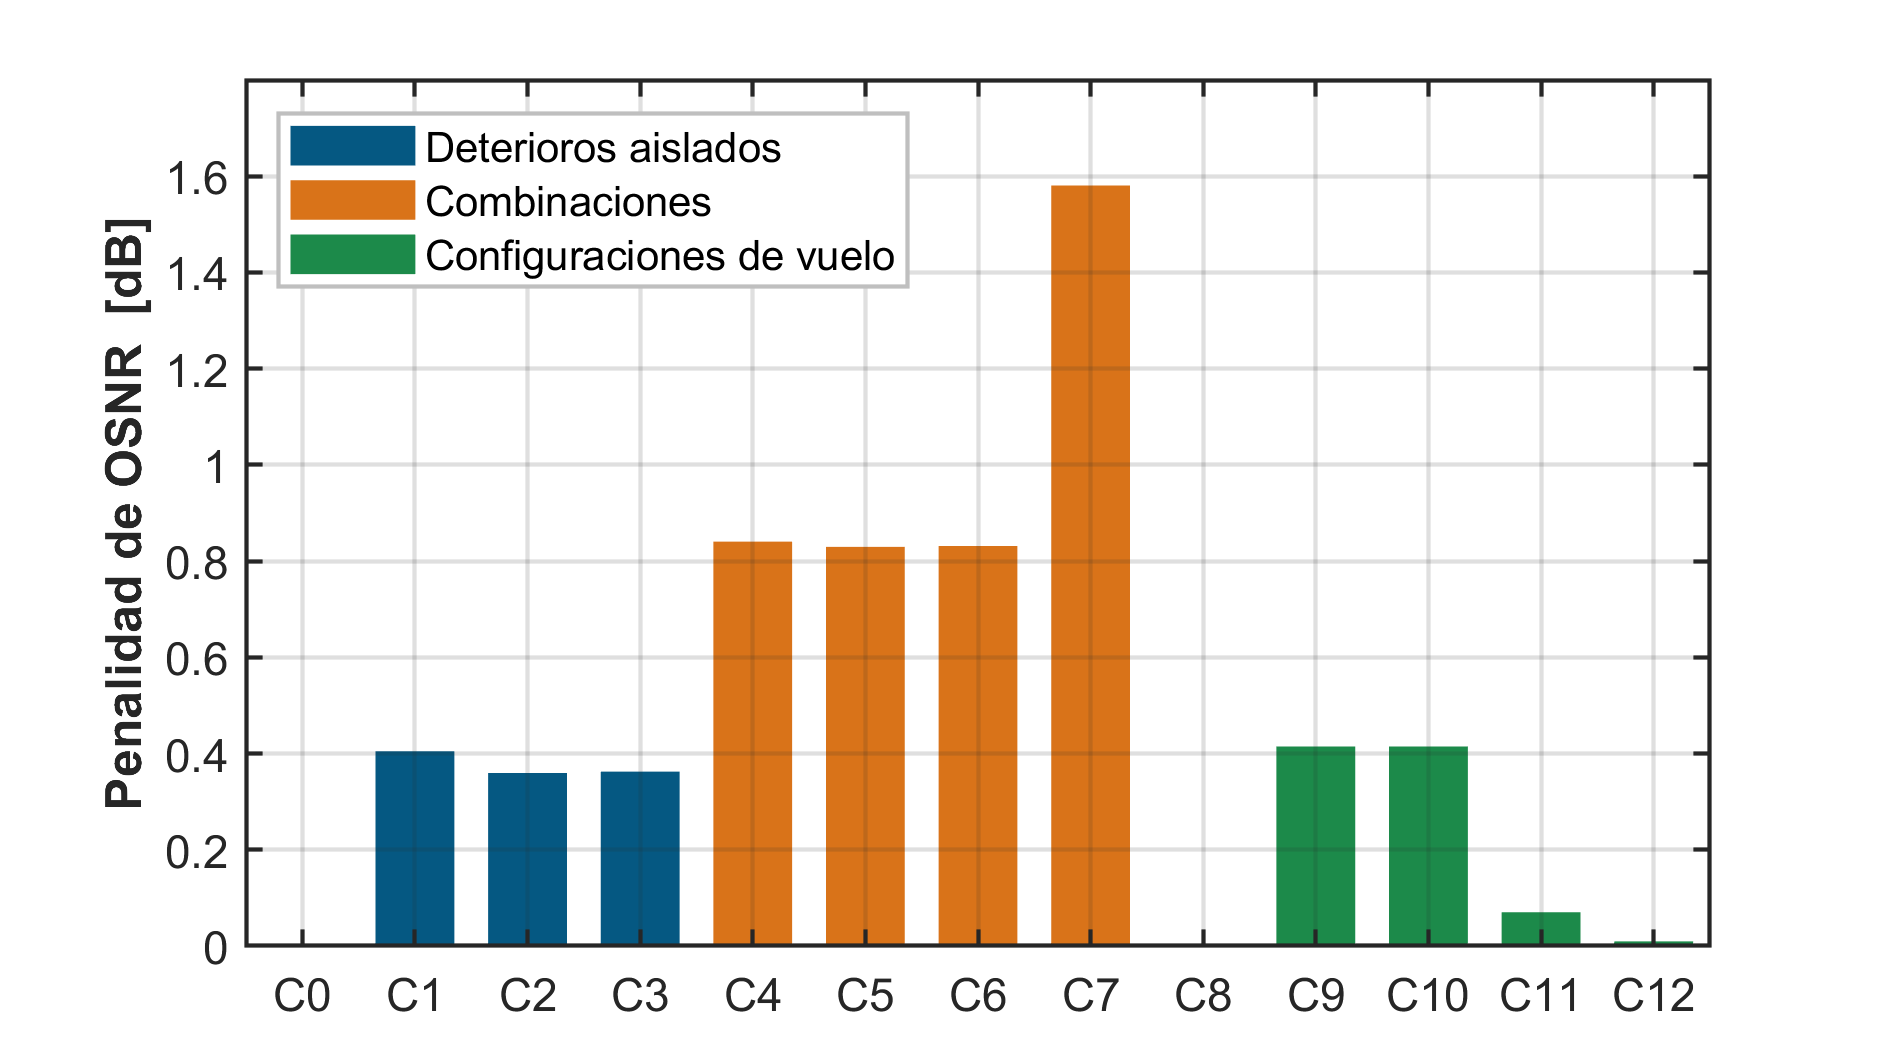
\includegraphics[width=0.95\textwidth]{figuras/tol_penalidad_configuraciones.png}
  \caption[Penalidad de OSNR por configuraci\'on]{%
    Penalidad de OSNR en el cruce del umbral HD-FEC, por configuraci\'on,
    respecto de \Cfg{0}. Los tres deterioros calibrados de \Cfg{1} a \Cfg{3}
    entran con el mismo peso, los pares de \Cfg{4} a \Cfg{6} son aditivos y
    \Cfg{7} es superaditiva.}
  \label{fig:tol-penalidad}
\end{figure}

La distancia entre el cruce medido y el de \Cfg{0} es lo que cuesta la
configuraci\'on. Estos valores se muestran en la \cref{fig:tol-penalidad} y en la
\cref{tab:tol-presupuesto}.

\begin{table}[htbp]
  \centering

  \begin{tabular}{llcc}
    \toprule
    & Deterioros activos & $\OSNR$ de cruce & Penalidad \\
    \midrule
    \Cfg{0}  & ninguno                   & \SI{13.18}{\dB} & ---             \\
    \midrule
    \Cfg{1}  & ancho de l\'inea          & \SI{13.58}{\dB} & \SI{0.40}{\dB}  \\
    \Cfg{2}  & deriva de polarizaci\'on  & \SI{13.54}{\dB} & \SI{0.36}{\dB}  \\
    \Cfg{3}  & skew                      & \SI{13.54}{\dB} & \SI{0.36}{\dB}  \\
    \midrule
    \Cfg{4}  & ancho de l\'inea y SOP    & \SI{14.02}{\dB} & \SI{0.84}{\dB}  \\
    \Cfg{5}  & ancho de l\'inea y skew   & \SI{14.01}{\dB} & \SI{0.83}{\dB}  \\
    \Cfg{6}  & SOP y skew                & \SI{14.01}{\dB} & \SI{0.83}{\dB}  \\
    \Cfg{7}  & los tres                  & \SI{14.76}{\dB} & \SI{1.58}{\dB}  \\
    \midrule
    \Cfg{8}  & vuelo, los que var\'ian   & \SI{13.18}{\dB} & \SI{0.00}{\dB}  \\
    \Cfg{9}  & vuelo, los fijos          & \SI{13.59}{\dB} & \SI{0.41}{\dB}  \\
    \Cfg{10} & vuelo completo            & \SI{13.59}{\dB} & \SI{0.41}{\dB}  \\
    \Cfg{11} & vuelo, skew \SI{2}{\pico\second} & \SI{13.25}{\dB} & \SI{0.07}{\dB} \\
    \Cfg{12} & vuelo, skew \SI{0}{\pico\second} & \SI{13.19}{\dB} & \SI{0.01}{\dB} \\
    \bottomrule
  \end{tabular}
  \caption[Presupuesto conjunto de deterioros]{%
    OSNR a la que cruza el umbral HD-FEC cada una de las configuraciones de
    la \cref{tab:tol-configs}, y penalidad respecto de \Cfg{0}.}
  \label{tab:tol-presupuesto}
\end{table}

De la tabla salen cuatro resultados.
\begin{puntos}
  \item La calibraci\'on cumple su prop\'osito: \Cfg{1}, \Cfg{2} y \Cfg{3}
        dan \num{0.40}, \num{0.36} y \SI{0.36}{\dB}. Los tres deterioros
        aislados pesan casi lo mismo, que era la condici\'on para poder
        compararlos de igual a igual.

  \item Los pares se apartan ligeramente de la suma lineal: \Cfg{4}, \Cfg{5} y
        \Cfg{6} dan \num{0.84}, \num{0.83} y \SI{0.83}{\dB}, contra los
        \SIrange{0.72}{0.76}{\dB} que predice la suma. El
        exceso ronda la d\'ecima de decibel en los tres casos. Se hace notar tambi\'en
        que los tres pares coinciden entre s\'i, lo que dice que ninguna
        combinaci\'on tiene mayor peso.

  \item Con los tres juntos el exceso se vuelve mayor: \Cfg{7} cuesta
        \SI{1.58}{\dB} contra \SI{1.12}{\dB} de la suma lineal.  Esto puede
        deberse a que los tres se corrigen con lazos que dependen de la
        decisi\'on. Cuando uno de ellos empeora las decisiones, los otros dos
        adaptan peor.

  \item El peor caso de vuelo es dominado por el skew: \Cfg{8} agrega la deriva de polarizaci\'on del pase y
        \SI{3}{\degree} de error de cuadratura. El resultado en este caso es id\'entico 
        al de \Cfg{0} en las nueve OSNR, porque la deriva real est\'a
        diez \'ordenes por debajo del quiebre y el error de cuadratura lo
        invierte la ortogonalizaci\'on. \Cfg{9} tiene una penalidad de \SI{0.41}{\dB}, todo debido al skew. 
        Sin skew, que es \Cfg{12}, la
        penalidad cae a \SI{0.01}{\dB}. Con \SI{2}{\pico\second}, que es
        \Cfg{11}, queda en \SI{0.07}{\dB}. Por eso \Cfg{9} y \Cfg{10} dan el
        mismo n\'umero. Lo que \Cfg{10} agrega sobre \Cfg{9} es justamente lo
        que \Cfg{8} muestra que no tiene penalidad.
\end{puntos}

\begin{figure}[H]
  \centering
  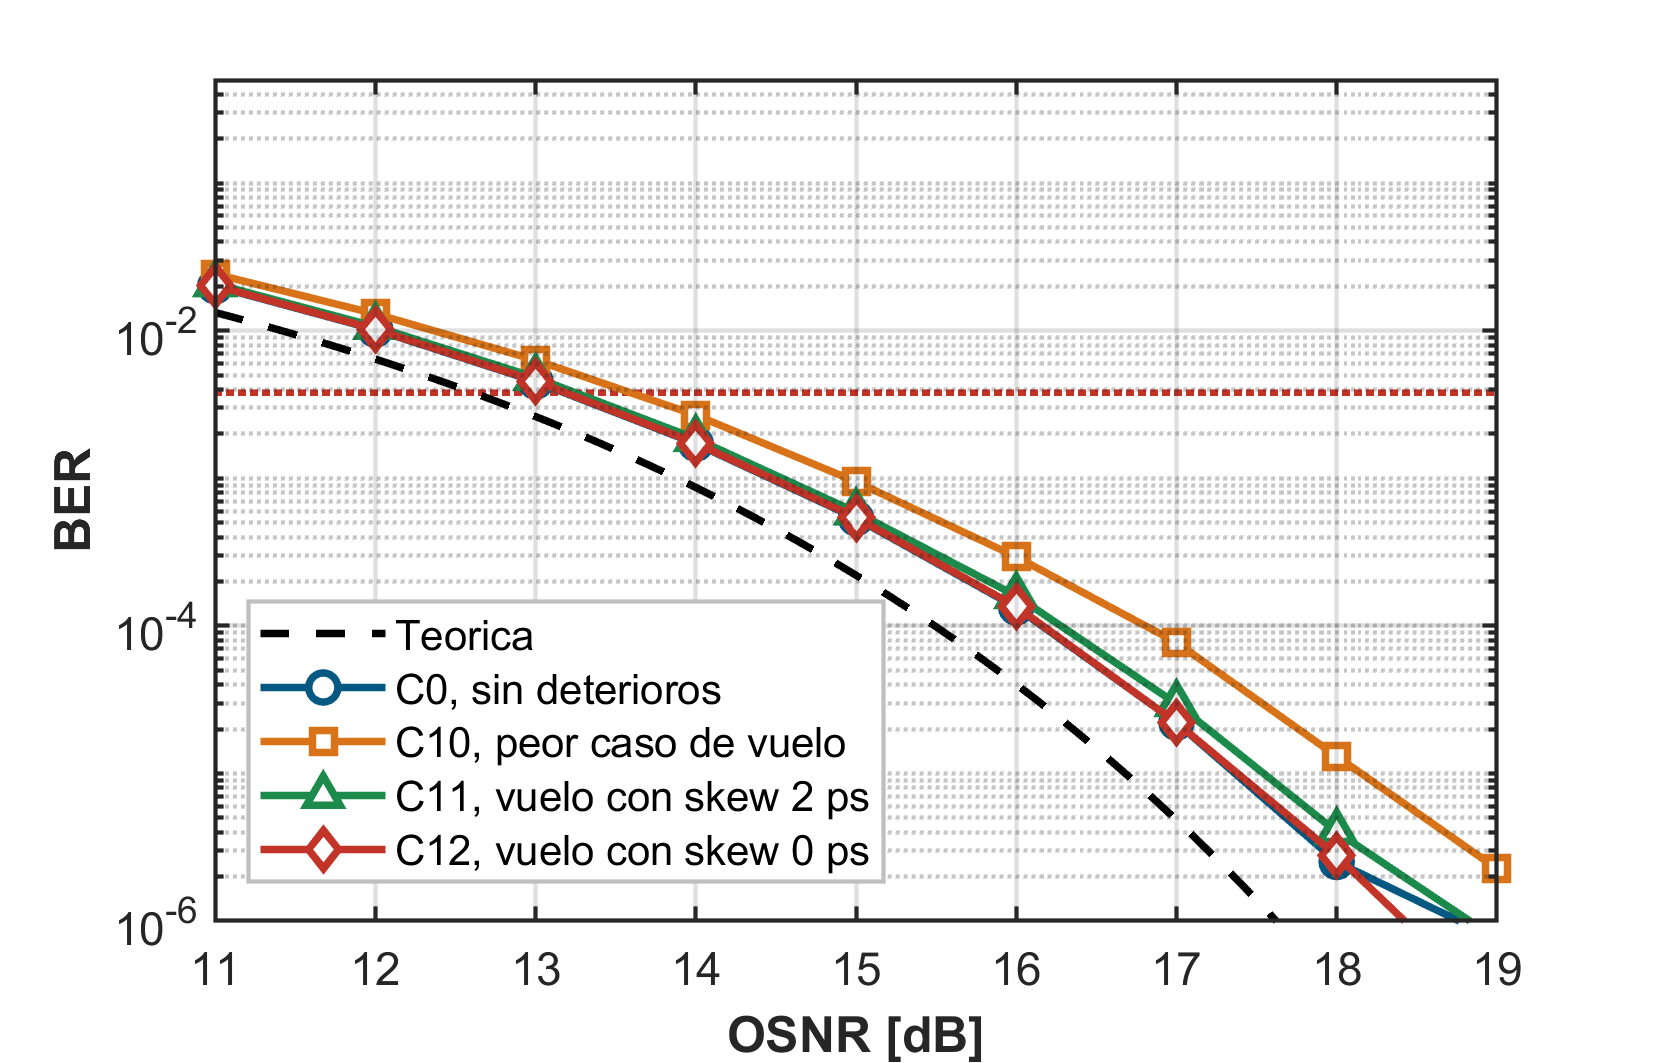
\includegraphics[width=0.85\textwidth]{figuras/tol_vuelo_ber_vs_osnr.png}
  \caption[Configuraciones de vuelo contra el receptor sin deterioros]{%
    BER contra OSNR de \Cfg{10}, \Cfg{11} y \Cfg{12}, comparadas con \Cfg{0} y
    con la curva te\'orica de DP-QPSK. La separaci\'on entre \Cfg{10} y
    \Cfg{0} es de \SI{0.41}{\dB} en el umbral, y desaparece casi por completo
    al reducir el skew del front end. La distancia entre la curva te\'orica y
    \Cfg{0} es la penalidad de implementaci\'on.}
  \label{fig:tol-vuelo}
\end{figure}

La \cref{fig:tol-vuelo} muestra las curvas BER para las tres \'ultimas configuraciones. Con el skew calibrado, el
ancho de l\'inea y la deriva de polarizaci\'on de especificaci\'on no imponen una penalidad significativa. El skew es el \'unico deterioro que importa en el presupuesto de vuelo,
lo que refuerza el requisito de calibraci\'on de la
\cref{sec:tol-frontend}.


\section{Conclusiones}
\label{sec:tol-conclusiones}

La \cref{tab:tol-final} re\'une todo el cap\'itulo. En ella se muestra, para cada deterioro, el
valor que impone el canal o el componente, la tolerancia medida y el margen
entre los dos.

\begin{table}[htbp]
  \centering

  \begin{tabular}{llll}
    \toprule
    Deterioro & Valor del enlace & Tolerancia medida & Margen \\
    \midrule
    Offset Doppler            & \SI{\pm 6.0}{\giga\hertz}          & \SI{\pm 8.0}{\giga\hertz}        & \SI{\pm 2.0}{\giga\hertz}    \\
    Chirp Doppler             & \SI{6.55}{\mega\hertz\per\second}  & \SI{1.8e12}{\hertz\per\second}   & \num{2.7e5}  \\
    Deriva de SOP             & \SI{1e-3}{\radian\per\second}       & \SI{2.15e7}{\radian\per\second}  & \num{2.2e10} \\
    Ancho de l\'inea          & \SI{100}{\kilo\hertz}              & \SI{3.16}{\mega\hertz}           & \num{32}     \\
    Error de reloj            & \SI{25.55}{\ppm}        & \SI{175}{\ppm}        & \num{6.8}    \\
    Skew del front end$^{*}$  & \SI{5}{\pico\second}               & \SI{4.5}{\pico\second}           & \num{0.9}    \\
    Fase de muestreo$^{*}$    & $0{,}25\,\Ts$                     & $>1{,}0\,\Ts$                 & $>\num{4}$   \\
    Error de cuadratura$^{*}$ & \SI{3}{\degree}                    & $>\SI{18}{\degree}$              & $>\num{6}$   \\
    \bottomrule
  \end{tabular}
  \caption[Resumen de tolerancias y m\'argenes]{%
    Tolerancia medida de cada deterioro contra el valor que impone el enlace.
    El margen es el cociente entre los dos. Los deterioros marcados con
    asterisco son calibrables en la integraci\'on y no propiedades del canal.}
  \label{tab:tol-final}
\end{table}

Se obtienen las siguientes conclusiones:

En primer lugar, el receptor tiene margen de sobra contra todo lo que impone
el canal. El deterioro m\'as ajustado de los provenientes del enlace es el
offset Doppler, con un margen de \SI{\pm 2.0}{\giga\hertz} sobre el requisito de \SI{\pm 6.0}{\giga\hertz}, y el resto est\'a entre uno y diez
\'ordenes de magnitud por encima del valor f\'isico. Ning\'un deterioro del
canal satelital amenaza el funcionamiento del receptor a
\SI{32}{\giga\baud}.

Por otro lado, el \'unico margen realmente estrecho no viene del canal sino
del equipo del receptor. El skew entre las ramas del front end tolera
\SI{4.5}{\pico\second} contra los \SI{5}{\pico\second} de especificaci\'on, es
decir que est\'a en el l\'imite, y es adem\'as el t\'ermino que domina el
presupuesto de vuelo de la \cref{sec:tol-presupuesto}. Reducir el skew a \SI{2}{\pico\second} en la integraci\'on disminuir\'ia la penalidad total de vuelo de \num{0.41} a \SI{0.07}{\dB}, lo cual ser\'ia recomendable en la pr\'actica.

En tercer lugar, el l\'imite de captura de Doppler, que es el margen m\'as
ajustado del lado del canal, es lo que justifica la tasa de s\'imbolo elegida.
Las tres tasas presentan un l\'imite en $\Rs/4$, de modo que la ventana de captura crece con
la tasa, y s\'olo \SI{32}{\giga\baud} cubre el requisito de
\SI{\pm 6.0}{\giga\hertz} con margen. 

Por \'ultimo, los dos deterioros que vienen del movimiento del sat\'elite, el
offset y el chirp, se barrieron contra una familia de doce valores de OSNR y
en ninguno de los dos el quiebre se vio afectado por el ruido. La
\cref{fig:tol-frecuencia-estimada} muestra adem\'as que el estimador de
frecuencia sigue el offset sin error apreciable hasta el \'ultimo punto
te\'orico posible, y que pasado el l\'imite salta al valor que predice el
plegado de Nyquist. Esto significa que estas tolerancias no son un compromiso
entre se\~nal y ruido que se pueda compensar con potencia \'optica. Son
propiedades de los algoritmos y de la frecuencia a la que se los utiliza.
Ampliar estas tolerancias exige cambiar el procesamiento, subiendo las
muestras por s\'imbolo o reemplazando el elevado a la cuarta por un m\'etodo
sin ambig\"uedad, no mejorando el enlace \'optico.

En cambio, los ruidos del l\'aser se comportan diferente. Tanto el de fase como el de
intensidad degradan el desempe\~no de forma gradual, y sus l\'imites var\'ian con la
OSNR, porque la falla ocurre cuando el deterioro y el ruido \'optico juntos
agotan el presupuesto de error. En esos dos casos la potencia \'optica implica un aumento de la tolerancia. Con el ancho de banda del lazo adoptado, el receptor admite
\SI{3.16}{\mega\hertz} de ancho de l\'inea por l\'aser, un factor \num{32}
sobre el requisito, y el RIN no impone ninguna restricci\'on en todo el rango
simulado. 

